\documentclass[11pt]{article}
% CS 6001 final report. All numbers come from assets/numbers.tex, generated by scripts/make_report_assets.py.
\usepackage[margin=1in]{geometry}
\usepackage{amsmath,amssymb,amsthm}
\usepackage{graphicx}
\usepackage[table]{xcolor}
\usepackage{tikz}
\usepackage[labelsep=period,font=small]{caption}
\usepackage[colorlinks=true,linkcolor=blue,citecolor=blue,urlcolor=blue]{hyperref}
\usepackage{parskip}
\usepackage{tabularx,pgfplots,makecell}
\usetikzlibrary{calc}
\pgfplotsset{compat=1.18}
\newcolumntype{Y}{>{\raggedright\arraybackslash}X}
\renewcommand{\arraystretch}{1.12}
% AUTO-GENERATED by scripts/make_report_assets.py: do not edit by hand
\newcommand{\DailyVol}{4.57\%}
\newcommand{\NReturns}{3,331}
\newcommand{\FeeBp}{5}
\newcommand{\CostBp}{1}
\newcommand{\SurplusBp}{10}
\newcommand{\QK}{100}
\newcommand{\DesignerK}{41}
\newcommand{\NTests}{196}
\newcommand{\NMutants}{12}
\newcommand{\VolSource}{DATA}
\newcommand{\FstarKTen}{0.083\%}
\newcommand{\FstarKHundred}{0.551\%}
\newcommand{\FstarKFourHundred}{1.425\%}
\newcommand{\FstarSizeSmall}{0.064\%}
\newcommand{\FstarSizeOne}{0.551\%}
\newcommand{\FstarSizeLarge}{1.443\%}
\newcommand{\VolSweepFactor}{8}
\newcommand{\VolSweepRatio}{27}
\newcommand{\WindowMinutes}{20}
\newcommand{\NFeasible}{25}
\newcommand{\NCells}{40}
\newcommand{\KappaAssumed}{1\%}
\newcommand{\KappaMax}{5.4\%}
\newcommand{\VolLow}{3.53\%}
\newcommand{\VolHigh}{5.61\%}
\newcommand{\FstarLow}{0.39\%}
\newcommand{\FstarHigh}{0.74\%}
\newcommand{\SpecPlainLow}{14.1}
\newcommand{\SpecPlainHigh}{23.8}
\newcommand{\FstarRatio}{1.9}
\newcommand{\SpecPlain}{18.9}
\newcommand{\SpecSmall}{11.1}
\newcommand{\SpecLarge}{$-3.3$}
\newcommand{\SpecFallback}{$-5.0$}
\newcommand{\SpecProducer}{11.1}
\newcommand{\SpecOptional}{11.1}
\newcommand{\SpecSelf}{18.9}
\newcommand{\WindowVol}{0.54\%}
\newcommand{\FstarWindow}{0.551\%}
\newcommand{\CoalBurnHalf}{10.4}
\newcommand{\CoalBurnOne}{4.2}
\newcommand{\CoalBurnThree}{0.013}
\newcommand{\CoalSelfMin}{21.4}
\newcommand{\CoalSelfMax}{21.4}
\newcommand{\CoalPoolMax}{0.40}
\newcommand{\CoalProdHalf}{1.7}
\newcommand{\CoalProdThree}{21.2}
\newcommand{\ThreshProducer}{0.050\%}
\newcommand{\ThreshPool}{0.200\%}
\newcommand{\DesNoForfeit}{0}
\newcommand{\DesPartial}{0}
\newcommand{\DesFull}{36}
\newcommand{\DesWindowVol}{0.341\%}
\newcommand{\DesFstarBp}{28.2}
\newcommand{\HanMaxDiff}{$10^{-13}$}
\newcommand{\ContestVo}{1}
\newcommand{\ContestKappa}{0.01}
\newcommand{\ContestCr}{0.002}
\newcommand{\ContestCap}{1}
\newcommand{\ContestRaceTies}{1}
\newcommand{\ContestRaceDeterCells}{2}
\newcommand{\ContestCells}{12}
\newcommand{\ContestBondFeasible}{11}
\newcommand{\ContestBondDeters}{11}
\newcommand{\ContestStrongRaceDeter}{0}
\newcommand{\ContestStrongBondDeter}{3}
\newcommand{\ContestStrongN}{3}
\newcommand{\RotCFdev}{$10^{-8}$}
\newcommand{\RotCells}{19}
\newcommand{\RotHalfFour}{8}
\newcommand{\RotHalfTwelve}{2,048}
\newcommand{\ThmN}{710}
\newcommand{\ThmAllPositive}{all}
\newcommand{\ThmMinMargin}{-7.7e-13}
\newcommand{\ThmMaxTotal}{$10^{-12}$}
\newcommand{\ImpBurnAll}{23}
\newcommand{\ImpPoolAll}{0}
\newcommand{\ImpProdAll}{0}
\newcommand{\ImpSelfAll}{0}
\newcommand{\ImpMixedAll}{0}
\newcommand{\ImpPerRouting}{300}
\newcommand{\BPLow}{2.03}
\newcommand{\BPHigh}{2.14}
\newcommand{\BPEpsLooseLow}{1.25}
\newcommand{\BPEpsLooseHigh}{1.32}
\newcommand{\BPExactLow}{5.5}
\newcommand{\BPExactHigh}{7.0}
\newcommand{\BPPartOpt}{0.45}
\newcommand{\BPCutoff}{5}
\newcommand{\BPFstarBp}{28.2}
\newcommand{\BPWindowVol}{0.34\%}
\newcommand{\HaveCI}{1}
\newcommand{\VolCI}{4.23\%--4.98\%}
\newcommand{\FstarCI}{0.49\%--0.63\%}
\newcommand{\HaveEmp}{1}
\newcommand{\EmpWindow}{20}
\newcommand{\EmpKurt}{52.8}
\newcommand{\EmpFstar}{0.158\%}
\newcommand{\EmpStepKurt}{121.2}
\newcommand{\EmpCI}{0.141\%--0.178\%}
\newcommand{\EmpWindowVol}{0.30\%}
\newcommand{\EmpNWindows}{86,380}
\newcommand{\EmpFrom}{2 August 2026}
\newcommand{\EmpTo}{1 October 2026}
\newcommand{\EmpImpliedDaily}{2.6\%}
\newcommand{\EmpLognormal}{0.236\%}
\newcommand{\EmpRatio}{0.67}
\newcommand{\HaveTwelve}{1}
\newcommand{\TwN}{100,700}
\newcommand{\TwWindowVol}{0.28\%}
\newcommand{\TwKurt}{11.0}
\newcommand{\TwStepKurt}{34.7}
\newcommand{\TwZeroShare}{12\%}
\newcommand{\TwFstar}{0.169\%}
\newcommand{\TwCI}{0.136\%--0.214\%}
\newcommand{\TwLognormal}{0.212\%}
\newcommand{\TwRatio}{0.80}
\newcommand{\TwFrom}{9 October}
\newcommand{\TwTo}{22 October 2026}
\newcommand{\TwSigmaStep}{0.0272\%}
\newcommand{\TwImpliedStep}{0.0538\%}
\newcommand{\TwBlockRatio}{0.51}
\newcommand{\TwDailyEq}{2.3\%}
\newcommand{\TwVRTwo}{1.05}
\newcommand{\TwVRLow}{1.08}
\newcommand{\TwVRHigh}{1.11}
\newcommand{\TwVRWindow}{1.08}
\newcommand{\TwZWindow}{2.3}
\newcommand{\TwUnderstate}{4\%}
\newcommand{\TwSigMinutes}{5}
\newcommand{\TwZRobWindow}{1.2}
\newcommand{\TwZRobSig}{2.3}
\newcommand{\TwZRobShort}{4.8}
\newcommand{\TwNBoot}{1,000}
\newcommand{\TwSeed}{0}
\newcommand{\HaveAssets}{1}
\newcommand{\AssetFLow}{0.39\%}
\newcommand{\AssetFHigh}{0.80\%}
\newcommand{\GaussFstar}{0.554\%}
\newcommand{\FeeLowF}{0.91\%}
\newcommand{\FeeHighF}{0.23\%}
\newcommand{\CommitFeeFive}{0.34\%}
\newcommand{\GaussMaxRelErr}{0.9\%}
\newcommand{\CpRatioHundred}{2.4}
\newcommand{\CpHundred}{1.35\%}
\newcommand{\CpFifty}{0.91\%}
\newcommand{\CpTwoHundred}{1.98\%}
\newcommand{\CpTen}{0.34\%}
\newcommand{\NBurnInfeasible}{6}
\newcommand{\NBurnCells}{15}
\newcommand{\FrontierK}{59}
\newcommand{\FrontierMin}{11.8}
\newcommand{\FrontierEightK}{20}
\newcommand{\FrontierEightMin}{4.0}
\newcommand{\FrontierTwoK}{307}
\newcommand{\FrontierTwoMin}{61.4}
\newcommand{\CpTolOne}{0.91\%}
\newcommand{\CpTolHundredth}{1.69\%}
\newcommand{\CpTolThousandth}{1.99\%}
\newcommand{\FrontierTolOneMin}{23.4}
\newcommand{\FrontierTolHundredthMin}{7.8}
\newcommand{\PoolN}{35}
\newcommand{\PoolF}{1.39\%}
\newcommand{\PoolExt}{1.75\%}
\newcommand{\PoolNoExt}{1}
\newcommand{\BPStepsLow}{5}
\newcommand{\BPStepsHigh}{80}
\newcommand{\BPEpsCoarse}{0.94}
\newcommand{\BPEpsFine}{2.15}
\newcommand{\BPEpsFineLow}{2.11}
\newcommand{\BPExactCoarse}{1.0}
\newcommand{\BPExactFine}{12.2}
\newcommand{\BPGridCoarse}{2.25}
\newcommand{\BPGridFine}{2.13}
\newcommand{\BPGridFineLowQ}{2.03}
\newcommand{\BPSensLo}{1.80}
\newcommand{\BPSensHi}{2.35}
\newcommand{\BPSensPriors}{4}
\newcommand{\BPSensWeights}{3}
\newcommand{\RobSettings}{12}
\newcommand{\RobStrongRace}{0}
\newcommand{\RobStrongBond}{12}
\newcommand{\RobRaceTiesMax}{1}
\newcommand{\SizePropMaxResidual}{4.2}
\newcommand{\SizeLineOverSmall}{23}
\newcommand{\SizePropFeeSpread}{0.0}
\newcommand{\QfZero}{0.551\%}
\newcommand{\QfSix}{0.540\%}
\newcommand{\QfNine}{0.475\%}
\newcommand{\HonestMaxLossBp}{0.00}
\newcommand{\HonestDropMax}{$1.1\times10^{-22}$}
\newcommand{\CentNash}{4}
\newcommand{\CentSPNE}{1}
\newcommand{\BurnNash}{25}
\newcommand{\BurnSPNE}{4}
\newcommand{\BurnNonCred}{21}
\newcommand{\ProdNash}{16}
\newcommand{\ProdSPNE}{1}
\newcommand{\HandV}{26.3333}
\newcommand{\PlainGainChecker}{7.76}
\newcommand{\ObsTwoRows}{9}
\newcommand{\ObsTwoDiff}{$10^{-13}$}

\renewcommand{\VolCI}{4.23\% to 4.98\%}\renewcommand{\FstarCI}{0.49\% to 0.63\%}\renewcommand{\EmpCI}{0.141\% to 0.178\%}\renewcommand{\TwCI}{0.136\% to 0.214\%}
\newtheorem{proposition}{Proposition}
\newcommand{\E}{\mathbb{E}}
\newenvironment{steps}{\begin{list}{}{\setlength{\leftmargin}{3.6em}\setlength{\labelwidth}{3.2em}\setlength{\labelsep}{0.4em}\setlength{\itemsep}{2pt}\setlength{\topsep}{3pt}\setlength{\parsep}{0pt}\renewcommand{\makelabel}[1]{##1\hfil}}}{\end{list}}
\setlength{\parskip}{3pt}
\setlength{\textfloatsep}{8pt plus 2pt minus 2pt}
\setlength{\floatsep}{6pt plus 2pt minus 2pt}
\setlength{\intextsep}{6pt plus 2pt minus 2pt}
\newcommand{\repo}{\url{https://github.com/reman-krishnan/cs6001-project}}

\title{Commit Now, Walk Away Later\\ Designing Forfeits for Delayed Blockchain Transactions\\ \large CS 6001 Course Project Final Report}
\author{Reman Krishnan (Roll No.\ 26D0365)}
\date{}

\begin{document}
\maketitle

\begin{abstract}
A blockchain serves as a shared record of signed transactions, where digital signatures verify each owner's approval. Current standardized quantum-resistant signatures are approximately 38 times larger than those used today. As a result, newer blockchain designs propose keeping these signatures off-chain, allowing users to authorize a committed transaction a few blocks later. This delay, however, provides users with a free option that enables them to abandon a bad trade. Existing penalties do not account for this option and overlook a producer who possesses the complete signature and can either publish it or collude with the user. This issue is formulated as a mechanism design problem, determining an appropriate forfeit, its intended recipient, and a producer fallback that discourages speculation, keeps both parties aligned, limits collusion, and minimizes collateral requirements. The resulting extensive-form game is solved for subgame-perfect equilibria and calibrated to nine years of ether price data. On its own, a forfeit needs to be between 0.39\% and 0.74\% of a trade over a span of 20 minutes. A credible fallback eliminates the option, but limiting collusion requires some of the forfeit to leave the user and producer. Sending all of it outside, for example by burning, is cheapest. At 20 minutes, burning 1.35\% of the trade keeps their joint gain over the best equilibrium within 0.1 basis points. However, a collateral cap of 1\% restricts the time window to a maximum of 11.8 minutes. Within this model, delayed authorization can achieve the stated incentive constraints, although the feasible window decreases as market volatility increases.
\end{abstract}

\section{Introduction}
A blockchain is a shared ledger, a list of transactions of which many independent computers, called nodes, keep identical copies. The ledger grows in batches called blocks, about one every twelve seconds on Ethereum. For each block one participant, the \emph{block producer}, chooses which waiting transactions to include and earns a fee for each. Every transaction carries a digital signature, a piece of data that only the account owner can produce and that proves the owner approved the transaction. These signatures are about to grow much larger. A sufficiently large quantum computer would break the signature schemes in use today, and the ML-DSA-44 scheme that NIST standardized as a replacement produces signatures of 2,420 bytes, against 64 bytes for a raw P-256 ECDSA signature~\cite{fips204,fips186}. Since every node must receive, check and store every signature, this growth raises the cost of running a ledger for everyone.

One recent proposal avoids this cost by keeping the full signature off the ledger~\cite{finlowbates2026}. The user first posts a \emph{commitment}, a short fingerprint (a hash) of the transaction that fixes its contents without revealing them, and a few blocks later posts a short secret value that authorizes it. We call such designs \emph{deferred-authorization protocols}. Their resistance to forgery has been analysed~\cite{lie2026finality}. Similar delays create options to abandon an unfavourable trade in atomic swaps, which exchange coins across two blockchains~\cite{han2019optionality}, and in Ethereum's planned proposer-builder separation (ePBS), where a separate builder assembles each block~\cite{mazorra2025epbs}. A separate literature studies collusion, in which users and producers coordinate as a coalition through private agreements~\cite{roughgarden2021tfm,chungshi2023}.

The draft Ethereum Improvement Proposal EIP-8209 burns, that is destroys, a prepaid fee when a commitment is not revealed~\cite{eip8209}, and defences against front-running, where others jump ahead of a pending transaction, penalize non-reveal or allow it~\cite{canidio2023commitment}. Among the works studied, none sizes such a penalty from the option's value and decides where its money should go when the producer can publish the signature and collude with the user. Section~\ref{sec:related} compares these lines of work.

This gap matters because the delay itself creates the problem. Suppose a user commits to buy an asset for \$100{,}000 at today's price, for example from a seller whose quoted price stays valid until the window closes, and the price over the next twenty minutes moves with a standard deviation of $0.5\%$. If the price rises, the user authorizes and gains at the seller's expense, and if it falls, the user stays silent and loses nothing. The user therefore holds a \emph{free option}, the right but not the duty to trade at a fixed price after seeing how the price moved. Staying silent caps the loss at zero, as Figure~\ref{fig:overview}(b) shows for an illustrative fee of $0.05\%$, and a forfeit $f$, a penalty charged when the user walks away, lowers that floor to $-f$. This option is worth roughly \$200 per commitment before fees under a normal approximation, far more than a typical fee.

Two mitigations have been proposed, but each creates a new difficulty. A forfeit fails if it is too small, and if it is paid to the producer, the producer is tempted to delay an honest user until the window closes so that it can collect the forfeit. A \emph{fallback} lets the producer, which privately receives the user's full signature with the commitment, publish it if the user stays silent, so the large signature reaches the ledger only then. This removes the option, but the user and the producer may then agree in private that the producer stays silent when the price falls and that the two share the gain when it rises. Although the setting comes from blockchains, this is a classical mechanism-design problem, in which a designer who cannot observe the user's motive must use payments to deter a profitable deviation, while the agent who enforces the rules has interests of its own and may collude with the user.

\begin{figure}[htbp]\centering
\begin{minipage}[b]{0.6\textwidth}\centering
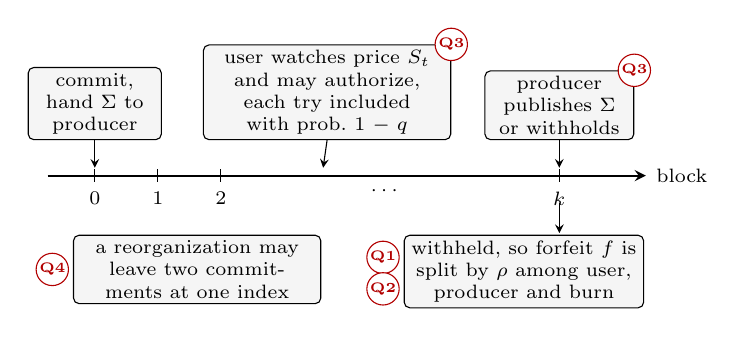
\begin{tikzpicture}[font=\scriptsize,>=stealth,
  box/.style={draw,rounded corners=2pt,align=center,inner sep=2pt,fill=gray!8},
  q/.style={circle,draw=red!70!black,text=red!70!black,font=\tiny\bfseries,inner sep=0.5pt,fill=white}]
\draw[->,thick] (0,0) -- (7.6,0) node[right]{block};
\foreach \x/\l in {0.6/0,1.4/1,2.2/2,6.5/$k$} \draw (\x,0.08)--(\x,-0.08) node[below=0pt]{\l};
\node at (4.3,-0.2){$\cdots$};
\node[box,anchor=south,text width=1.55cm] (c) at (0.6,0.45) {commit, hand $\Sigma$ to producer};
\node[box,anchor=south,text width=3.0cm] (w) at (3.55,0.45) {user watches price $S_t$ and may authorize, each try included with prob.\ $1-q$};
\node[box,anchor=south,text width=1.75cm] (p) at (6.5,0.45) {producer publishes $\Sigma$ or withholds};
\draw[->] (c.south)--(0.6,0.1); \draw[->] (w.south)--(3.5,0.1); \draw[->] (p.south)--(6.5,0.1);
\node[q] at ($(w.north east)+(0,0)$) {Q3};
\node[q] at ($(p.north east)+(0,0)$) {Q3};
\node[box,anchor=north,text width=2.9cm] (d) at (6.05,-0.75) {withheld, so forfeit $f$ is split by $\rho$ among user, producer and burn};
\draw[->] (6.5,-0.35) -- (6.5,-0.73);
\node[q,anchor=east] at ($(d.west)+(-0.05,0.18)$) {Q1};
\node[q,anchor=east] at ($(d.west)+(-0.05,-0.22)$) {Q2};
\node[box,anchor=north,text width=3.0cm] (r) at (1.9,-0.75) {a reorganization may leave two commitments at one index};
\node[q,anchor=east] at ($(r.west)+(-0.05,0)$) {Q4};
\end{tikzpicture}\\[-1pt]
{\footnotesize (a) Timeline of one commitment}
\end{minipage}\hfill
\begin{minipage}[b]{0.38\textwidth}\centering
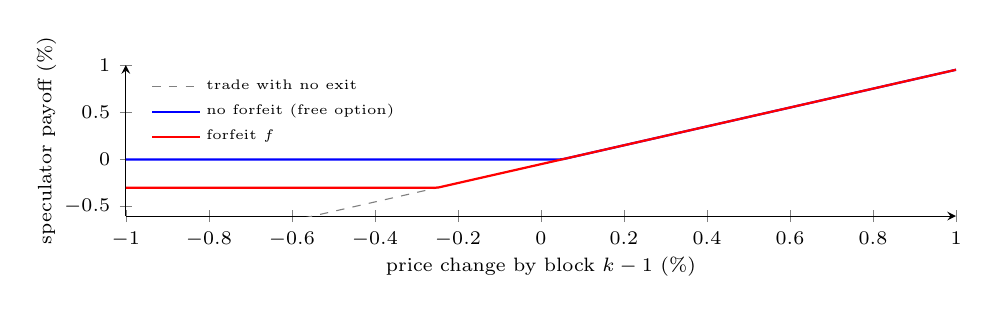
\begin{tikzpicture}
\begin{axis}[width=\linewidth,height=3.5cm,font=\scriptsize,
  xlabel={price change by block $k-1$ (\%)},ylabel={speculator payoff (\%)},
  xmin=-1,xmax=1,ymin=-0.6,ymax=1,axis lines=left,
  legend style={font=\tiny,at={(0.02,0.98)},anchor=north west,draw=none,fill=none},legend cell align=left,
  ylabel style={yshift=-4pt},xlabel style={yshift=3pt}]
\addplot[domain=-1:1,samples=3,gray,dashed] {x-0.05};
\addplot[domain=-1:1,samples=200,thick,blue] {max(x-0.05,0)};
\addplot[domain=-1:1,samples=200,thick,red] {max(x-0.05,-0.3)};
\legend{trade with no exit,no forfeit (free option),forfeit $f$}
\end{axis}
\end{tikzpicture}\\[-1pt]
{\footnotesize (b) Payoff of walking away}
\end{minipage}
\caption{The problem at a glance.}\label{fig:overview}
\end{figure}

The objective of this report is to find forfeit designs that remove the option while staying safe against producers and against collusion. The scope is the incentives around a single commitment, not the bandwidth the design saves. Within this scope it answers four questions, each marked in red where it arises on the timeline of Figure~\ref{fig:overview}(a). There $\Sigma$ is the user's full signature, $S_t$ the price at block $t$, $k$ the deadline block, $q$ the chance that an attempt is left out of a block, and $\rho$ the rule that splits $f$ among the user, the producer and burning. The last question concerns a reorganization, in which recent blocks are replaced and two commitments can end up on one \emph{index}, the numbered account slot that a commitment occupies.
\begin{itemize}\setlength{\itemsep}{0pt}
\item \textbf{Q1.} How small can a forfeit be and still remove the option, given the window, volatility and size?
\item \textbf{Q2.} Where should the forfeit go so that the producer still publishes and honest users are unharmed?
\item \textbf{Q3.} When can a producer, alone or together with the user, profit by keeping the option alive?
\item \textbf{Q4.} Should a dispute over an index be settled by a bonded contest or by a race?
\end{itemize}

To answer these questions, the protocol is modelled as a game in which the user and the producer move in turn and a chance player, nature, draws the price at each block. The designer's choice is then written as an optimization over mechanisms with deterrence, individual-rationality, credibility, collusion-proofness and collateral constraints. The game is solved by backward induction, finding each player's best action from the last block back to the first, with proofs where closed forms exist and numerical solutions elsewhere. The report contributes a game model with an independently checked solver, one main analytic result (an impossibility result for forfeits that stay with the user or producer), six shorter propositions, among them the optimality of burning, and calibrated answers to all four questions.

\section{Related Work}\label{sec:related}
Table~\ref{tab:related} lists the closest lines of work, what each establishes and what this report adds.

\begin{table}[htbp]\centering\scriptsize
\renewcommand{\arraystretch}{1.15}
\begin{tabularx}{\textwidth}{|>{\raggedright\arraybackslash}p{3.3cm}|Y|Y|}
\hline
\rowcolor{gray!15}Line of work & What it establishes & What this report adds \\
\hline
Game theory for blockchains~\cite{babaioff2012redballoons,eyal2014majority,kiayias2016mining,carlsten2016instability,huberman2021monopoly,leshno2020axiomatic} & Relaying, mining and fee markets are standard game-theoretic questions at top venues & The same tools applied to a delayed authorization \\
\hline
Transaction-fee mechanisms~\cite{roughgarden2021tfm,chungshi2023,chung2024collusion,gafni2024barriers} & Fee rules as mechanisms with user, miner and collusion constraints. EIP-1559 resists off-chain agreements (OCA-proofness) only because it burns its base fee & Collusion-proofness here is OCA-proofness for one user and one producer, and Proposition~\ref{prop:imposs} is its analogue for forfeits \\
\hline
Credible auctions with commitments~\cite{akbarpour2020credible,ferreira2020credible,chitra2024broadcast,ganesh2025matroids} & A bidder who commits but does not reveal pays a fine or loses collateral, sized to make the auction credible & Here the enforcer, the producer, can complete the transaction itself, and where the money goes matters \\
\hline
Deferred authorization~\cite{finlowbates2026,lie2026finality} & Commit first, authorize later, to keep large signatures off the ledger. A censoring adversary can forge unless eligibility is fixed before disclosure & Adds a fallback, a forfeit and a dispute rule, and asks what a producer \emph{wants} to do rather than what it \emph{can} do \\
\hline
Option value of delay~\cite{han2019optionality,crr1979,xu2021htlc,xue2021hedging,mazumdar2022quick,dubovitskaya2021packetized,mazorra2025epbs} & Atomic swaps and ePBS create free options, priced with the binomial lattice, and penalize the party that holds the option & Here a third party, the producer, can switch the option off or keep it alive by colluding \\
\hline
Hashed time-lock contract (HTLC) incentives and Rapidash~\cite{tsabary2021mad,wadhwa2023hehtlc,chung2025rapidash} & Miners enforce penalties or are bribed. Rapidash burns most funds, pays a small reward, and sets a $T$-block timeout so that a coalition with mining share $\gamma$ holds every block only with probability $\gamma^T$ & Pool routing and Proposition~\ref{prop:rot} rest on these ideas, applied to a producer that holds a usable signature under a collateral limit \\
\hline
Commit-reveal penalties in practice~\cite{eip8209,canidio2023commitment,lee2025commitreveal,sip80,eip8184} & Fees for not revealing are burned, pooled or slashed, at amounts fixed by rule & The penalty is sized from the value of the option \\
\hline
Payments and budget balance in mechanism design~\cite{vickrey1961,clarke1971,groves1973,greenlaffont1977,cavallo2006,guoconitzer2009,myerson1981} & Where collected money goes, and its tension with budget balance & The routing question, since money must leave the pair of user and producer \\
\hline
Producer extraction and disputes~\cite{daian2020flashboys,luu2015demystifying,kalodner2018arbitrum,mccorry2019pisa,baye1996allpay} & Producers profit from ordering, and disputes are settled by bonds or all-pay races & Bond and race compared for disputed indices (Q4), with ordering profits left for future work \\
\hline
\end{tabularx}
\caption{Related work and what this report adds.}\label{tab:related}
\end{table}

Burning against collusion, collateral for credible revelation and the window argument are therefore known, and what is new here is their combination for a producer that holds a usable signature.

\section{Model}\label{sec:model}
\textbf{Players, timeline and information.} The model follows one commitment, as in Figure~\ref{fig:overview}(a). The players are a user $U$, a block producer $P$ and nature, which is not strategic and stands for the randomness of the price. A block lasts twelve seconds, and the window $k$ is the number of blocks between the commitment and the deadline. At block $0$ the user commits and, when the protocol requires it, hands the full signature $\Sigma$ to the producer. The price $S_t$ at block $t$, with $S_0$ denoting the commitment-time price, follows a recombining binomial lattice, a tree in which an up-move followed by a down-move reaches the same price as the reverse, and in which the price moves up by the factor $u=e^{\sigma}$ or down by $d=1/u$ at each block, where $\sigma$ is the per-block volatility parameter controlling the size of price changes. After $j$ up-moves in $t$ blocks the price is $S_t=S_0e^{\sigma(2j-t)}$, and an up-move has probability $p=(1-d)/(u-d)$. This makes $S_t$ a martingale, meaning that the expected future price equals the current price. At blocks $1,\dots,k-1$ the user may attempt to authorize, and each attempt is included with probability $1-q$. Inclusion failures are independent of prices, and Q3 studies deliberate censorship separately. If the user has not authorized by block $k$, a producer holding $\Sigma$ chooses whether to publish it. If the producer withholds it, or never received it, the commitment is dropped and the user is charged the forfeit $f$. Every player sees all earlier moves before it acts, so this is an extensive-form game with perfect information and chance moves. Figure~\ref{fig:tree} draws it for $q=0$, when every authorization is included, with circles marked N for nature's price moves and payoffs written as (user, producer).

\textbf{Payoffs.} Outcomes are measured in money, and players are risk neutral with quasi-linear utilities, so they maximize expected money and a coalition can share its gain through transfers. The transaction has value $N$ and is priced at the commitment-time price $S_0$, so executing it at block $t$ is worth $g_t=N(S_t/S_0-1)$ to the user. On execution the user pays the producer a flat fee $\phi$, and publishing the signature costs the producer $c$. This payoff fits a fixed-price purchase from a seller who must honour the quote until the deadline, and other transaction types need their own payoff model. A speculator commits only for the option, while an honest user values execution at a constant $v$ with $v>\phi$, so its surplus from executing is $v-\phi$. Figure~\ref{fig:tree} gives the payoff of each outcome, and Table~\ref{tab:notation} lists the notation and the baseline values. Money is quoted as a fraction of $N$, and one basis point (bp) is $10^{-4}$ of $N$, or $0.01\%$. A routing rule $\rho=(\rho_U,\rho_P,\rho_O)$ splits a dropped forfeit into the shares returned to the user, paid to the producer and sent outside the pair, with $\rho_U+\rho_P+\rho_O=1$. Self is $(1,0,0)$, burn is $(0,0,1)$ and destroys the money, producer is $(0,1,0)$, and pool$(n)$ gives the producer $1/n$ and sends the rest outside the pair. The user locks $f$ as collateral until settlement. Execution returns this deposit, and a drop distributes it according to $\rho$. The collateral limit $\kappa_c$ caps the deposit at $\kappa_c N$.

\begin{figure}[htbp]\centering
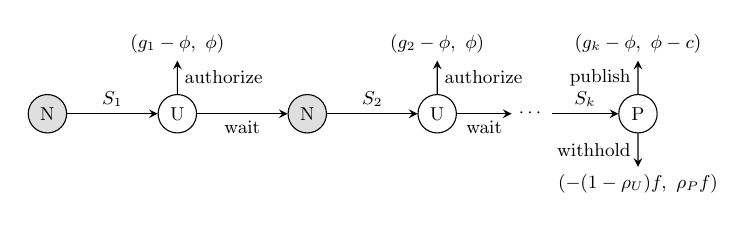
\begin{tikzpicture}[scale=0.75, transform shape, >=stealth, font=\small, dec/.style={circle,draw,minimum size=6.5mm,inner sep=0pt}, chance/.style={circle,draw,fill=gray!25,minimum size=6.5mm,inner sep=0pt}]
\node[chance] (n1) at (0,0) {N};
\node[dec] (u1) at (2.2,0) {U};
\node[chance] (n2) at (4.4,0) {N};
\node[dec] (u2) at (6.6,0) {U};
\node (dots) at (8.2,0) {$\cdots$};
\node[dec] (p) at (10,0) {P};
\draw[->] (n1) -- node[above]{$S_1$} (u1);
\draw[->] (u1) -- node[below]{wait} (n2);
\draw[->] (n2) -- node[above]{$S_2$} (u2);
\draw[->] (u2) -- node[below]{wait} (dots);
\draw[->] (dots) -- node[above]{$S_k$} (p);
\draw[->] (u1) -- node[right]{authorize} ++(0,0.9) node[above]{$(g_1-\phi,\ \phi)$};
\draw[->] (u2) -- node[right]{authorize} ++(0,0.9) node[above]{$(g_2-\phi,\ \phi)$};
\draw[->] (p) -- node[left]{publish} ++(0,0.9) node[above]{$(g_k-\phi,\ \phi-c)$};
\draw[->] (p) -- node[left]{withhold} ++(0,-0.9) node[below]{$(-(1-\rho_U)f,\ \rho_P f)$};
\end{tikzpicture}
\caption{The base game for $q=0$.}\label{fig:tree}
\end{figure}

\begin{table}[t]\centering\footnotesize
\begin{tabularx}{\textwidth}{|l|Y|l|}
\hline
\rowcolor{gray!15}Symbol & Meaning & Baseline value \\
\hline
$k$ & window length in 12-second blocks & \QK\ blocks (\WindowMinutes\ minutes) \\
\hline
$\sigma_{\text{day}}$ & daily volatility (standard deviation of daily log price changes) of ether & \DailyVol, interval \VolCI \\
\hline
$q$ & probability that an authorization attempt is censored, that is, left out & $0$, varied in Q1 \\
\hline
$N$, $\phi$ & transaction value, and flat fee paid to the producer on execution & one unit, \FeeBp\ bp \\
\hline
$c$, $v-\phi$ & producer's publishing cost, and honest user's surplus & \CostBp\ bp, \SurplusBp\ bp \\
\hline
$\rho=(\rho_U,\rho_P,\rho_O)$ & shares of $f$ to the user, the producer and outside the pair & self, burn, producer, pool$(n)$ \\
\hline
$f$, $\kappa_c$ & forfeit for an unauthorized commitment, and collateral limit as a fraction of $N$ & varied, \KappaAssumed \\
\hline
\end{tabularx}
\caption{Notation and baseline values.}\label{tab:notation}
\end{table}

\textbf{Threat model.} The threats are economic, not cryptographic. Every party acts in its own interest, and the signature and hash commitment are assumed secure~\cite{lie2026finality}. The producer earns only fees and its share of forfeits, and may censor attempts, withhold the signature, or agree with the user on an enforceable side payment. The committed transaction stays valid and executable throughout the window. The user cannot invalidate the fallback by moving funds, changing its transaction counter (nonce) or permissions, or cancelling, and the seller's quote or reserved assets keep the terms enforceable. Without these assumptions Proposition~\ref{prop:cred} would fail. Order profits, network attacks and larger coalitions are not modelled.

\textbf{Solution concept.} A strategy says what a player does at every decision point, even one never reached, and a pure strategy never randomizes. In a subgame-perfect Nash equilibrium (SPE), found by backward induction, no player gains by changing its own strategy after any history, which rules out threats a player would not carry out. Write $V_0$ for a user's expected payoff from committing, against zero for staying out. A design \emph{deters} speculation if the speculator's $V_0$ is at most $0$ in every pure SPE, where an indifferent speculator stays out and an indifferent producer may break its tie differently at each state. A coalition is the user and producer coordinating their actions and sharing the gain through private side payments. For a strategy profile $s$, the collection of all players' strategies, let $J(s)$ be the expected joint payoff of the user and producer, and let $J^*$ be the largest joint payoff they can reach over all joint strategies with side payments. A coalition's \emph{gain} is $\Delta=J^*-\max_s J(s)$, where the maximum runs over SPE with uniform tie-breaking, meaning that each kind of indifference is resolved by the same action at every node. With a strictly credible fallback, meaning that the producer earns strictly more by publishing than withholding, the equilibrium attaining this maximum is the \emph{honest} one, in which the user tries to authorize at every block, but the user is indifferent among authorization times. If it waits for the fallback, the producer always pays $c$ to publish rather than only when all $k-1$ attempts fail, so this waiting equilibrium has a joint payoff lower by $c(1-q^{k-1})$. When the producer prefers to withhold, the best equilibrium already involves strategic timing. Collusion guarantees are thus relative to the best equilibrium, not to every one.

\textbf{The designer's problem.} The question is one of mechanism design with transfers. A designer, whoever writes the protocol rules, fixes a mechanism $M=(k,f,\rho,\mathcal A)$ before play, where $\mathcal A$ states whether the producer may publish the signature and whether the user must hand it over. $M$ induces the extensive-form game above, an indirect and dynamic mechanism, and the aim is to implement in SPE an outcome in which speculators gain nothing by entering and honest users still want to participate~\cite{moore1988spi}. Write $V_0^{\mathrm{spec}}$ and $V_0^{\mathrm{hon}}$ for the values of committing to a speculator and to an honest user. With a collusion tolerance $\varepsilon\ge0$ and the collateral limit $\kappa_c$, the designer's program is
\begin{align*}
\min_{M}\ f\quad\text{subject to}\quad
&\text{(D)}\ \ V_0^{\mathrm{spec}}(M)\le 0\ \text{in every pure SPE} &&\text{deterrence}\\
&\text{(IR)}\ \ V_0^{\mathrm{hon}}(M)\ge 0 &&\text{individual rationality}\\
&\text{(CR)}\ \ \phi-c>\rho_P f\ \ \text{(designs with a fallback)} &&\text{credibility}\\
&\text{(CP}_\varepsilon\text{)}\ \ \Delta(M)\le\varepsilon &&\text{collusion-proofness}\\
&\text{(K)}\ \ f\le\kappa_c N &&\text{collateral.}
\end{align*}
The objective is the collateral an honest user must lock, and Table~\ref{tab:guarantees} in Appendix~\ref{app:choices} states exactly what (D) and (IR) promise. (CR) is the incentive constraint of the producer, the agent that enforces the rules, much as a credible auction needs an auctioneer who prefers to follow them~\cite{akbarpour2020credible}. (CP$_0$), the case $\varepsilon=0$, is OCA-proofness for one pair~\cite{roughgarden2021tfm} and plays the role of the coalition incentive constraint of collusion-proof mechanism design~\cite{laffont1997collusion}. The routing $\rho$ decides budget balance. A forfeit kept inside the pair ($\rho_O=0$) balances the pair's budget, while burning destroys money, as in money-burning mechanisms~\cite{hartline2008burning}. The questions solve restricted versions of this program. In each, collateral is minimized with the window fixed, and the largest feasible window is searched for separately. A credible fallback already meets (D) at $f=0$, so with a fallback the binding constraints are (CR), (CP$_\varepsilon$) and (K). Q1 fixes the window, rules out a fallback and finds the smallest burned forfeit meeting (D). Q2 asks which routings meet (CR) and (CP) together. Q3 fixes the window, requires a credible fallback, finds the cheapest routing and forfeit meeting (CP$_\varepsilon$), and then finds the largest window for which that forfeit meets (K). Q4 compares two rules for a related dispute. Appendix~\ref{app:choices} explains each modelling choice.

\textbf{Extensions.} Three extensions relax the base game. In the \emph{rotating-producer} model each block is produced, independently, by a strategic entity with probability $\alpha$ (its share of the blocks) and otherwise by an honest producer, so $\alpha=1$ is a single sequencer, the one operator that orders every block of a rollup, a chain that runs on top of Ethereum.

In the \emph{contest} model, a reorganization leaves two valid commitments at one index. An attacker with value $V_a$ and cost $\kappa$ rebinds the index, and the owner, who would lose $V_o$, is present with probability $a$. Under a \emph{bond} the attacker posts $b$. A present owner answers by posting a matching bond, which needs capital $K\ge b$, and showing the valid signature at a response cost $c_r$, which settles the claim in its favour, so it recovers its own bond and wins the attacker's. Under a \emph{race} both sides pay for priority even if they lose, an all-pay contest~\cite{baye1996allpay}.

In the \emph{private-type} model, each user has a hidden exposure $\theta$, an additional personal benefit of $\theta N$ from execution, and the designer balances the gain exposed users make by timing their authorization against the surplus of deterred users (Appendix~\ref{app:extra}). Offering users a menu of (window, forfeit) pairs to choose from, in the spirit of the revelation principle~\cite{myerson1979incentive}, is an open extension.

\section{Analytic Results}\label{sec:theory}
This section states Propositions~\ref{prop:self} to~\ref{prop:imposs}, of which Proposition~\ref{prop:imposs} is the main new result. The remaining three results and the full proofs of Propositions~\ref{prop:value} to~\ref{prop:route} appear in Appendix~\ref{app:proofs}. Propositions~\ref{prop:value} to~\ref{prop:imposs} use the martingale property $\E[g_{t+1}\mid S_t]=g_t$, where $\E$ denotes expectation and the vertical bar means conditioning on the current price. We write $x^+=\max(x,0)$.

\begin{proposition}[Self-routing is inert]\label{prop:self}
If the forfeit returns to the user, no payoff depends on $f$.
\end{proposition}
\emph{Proof.} The user's payoff on a dropped commitment is $-(1-\rho_U)f=0$, and no other payoff involves $f$. \hfill$\square$

The next result measures the option that remains when there is no fallback, and so answers Q1 in closed form.

\begin{proposition}[Value of the option]\label{prop:value}
Without a fallback, with $k\ge2$ and $q=0$, let the user lose $f$ when the commitment is dropped. Then the speculator's value is
\[V_0(f)=\E[\max(g_{k-1}-\phi,-f)]=-f+\E\big[(g_{k-1}-(\phi-f))^+\big]=\E\big[((\phi-f)-g_{k-1})^+\big]-\phi .\]
Speculation is deterred if and only if $\E[(g_{k-1}-(\phi-f))^+]\le f$. $V_0$ is continuous and non-increasing in $f$ and equals $-\phi\le0$ once $f\ge\phi-\min g_{k-1}$, so a smallest deterring forfeit $f^*$ exists whenever $V_0(0)>0$.
\end{proposition}
Because the price is a martingale, waiting leaves the expected trade value unchanged while keeping the choice to abandon an unfavourable trade, so waiting is worth at least authorizing early (Appendix~\ref{app:proofs}), so the speculator waits until the last block and authorizes only if the trade is then worth more than the fee minus the forfeit. Since a drop is always observed, this mirrors Becker's rule that a surely detected penalty must cover the expected gain from the offence~\cite{becker1968crime}, here the option's value. Ruling out early authorization parallels Merton's result that an American call, an option to buy at a fixed price at any time before expiry, is never exercised early on an asset that pays no dividends~\cite{merton1973}. The third form says that $f^*$ is the forfeit at which a put option on $g_{k-1}$ with strike $\phi-f$, a contract paying the amount by which $g_{k-1}$ ends below $\phi-f$, is worth exactly the fee $\phi$. The next result gives the condition under which the producer uses the fallback.

\begin{proposition}[Credibility threshold]\label{prop:cred}
With a fallback, no contestation and the signature handed over, the producer publishes at block $k$ if and only if $\phi-c>\rho_P f$, and it is indifferent at equality. If it publishes, then $V_0=-\phi$ for every $q\in[0,1]$ and every forfeit. If it withholds, the game is the one without a fallback.
\end{proposition}


The next result asks whether this credibility also prevents collusion.

\begin{proposition}[Forfeits that stay inside the pair]\label{prop:imposs}
Let there be a fallback with the signature handed over, $k\ge2$, $\sigma>0$, $q<1$ and no contestation, and let $\rho_O=0$. If the producer strictly prefers to publish, that is $\phi-c>\rho_P f$, then every equilibrium has a joint payoff of the user and producer of at most $0$, while a coalition with side payments can obtain at least $(1-q)\E[g_1^+]>0$. Such a design is therefore not collusion-proof.
\end{proposition}
\emph{Proof idea.} Under strict credibility every commitment executes, the fee cancels inside the pair, and by optional stopping the joint payoff of any equilibrium is at most $0$. Because the price is a martingale and execution happens by a fixed deadline, choosing when to execute cannot create a positive expected trading gain. The coalition instead authorizes at block $1$ only after a price rise and lets the producer withhold otherwise, which costs the pair nothing because $\rho_O=0$. The full proof is in Appendix~\ref{app:proofs}.


Strictness is needed, since at equality the outcome depends on tie-breaking. In mechanism-design terms, a forfeit that balances the budget of the pair cannot be both credible and collusion-proof, so some money must leave the pair. This is balance within the pair, not budget balance of a whole mechanism, so the result is an analogue of, not a derivation from, the classical tension between budget balance and other goals~\cite{greenlaffont1977,nath2019budget}, and it is closest to Roughgarden's case for burning the base fee.

A producer that receives part of the forfeit can also harm an honest user directly. It can refuse to include the user's authorization until the window closes and then withhold the signature, collecting the forfeit, which this report calls extortion, and Proposition~\ref{prop:rot} (Appendix~\ref{app:proofs}) gives its threshold under rotating producers.




\section{Experimental Framework}\label{sec:framework}
\textbf{Implementation and verification.} The propositions cover the cases with closed forms, and the rest come from a lattice solver, written in Python with NumPy and SciPy (\repo), that computes equilibria by backward induction over the price tree. It reproduces a hand-computed game, agrees with a separate game-tree solver, exhaustive enumeration and textbook binomial option prices, and passes all \NTests\ automated tests, which catch all \NMutants\ deliberately injected bugs (Table~\ref{tab:verify} in the appendix).


\textbf{Calibration.} Volatility is the root-mean-square daily log return (change in log price) of Binance's daily ether (ETH) closes in USDT, 17 August 2017 to 30 September 2026, giving $\sigma_{\text{day}}=\DailyVol$ from \NReturns\ returns with a $95\%$ moving-block bootstrap interval of \VolCI, which measures uncertainty by repeatedly resampling runs of consecutive days. The per-block volatility of Section~\ref{sec:model} is $\sigma=\sigma_{\text{day}}\sqrt{12/86400}$, which assumes uncorrelated log returns. The other values in Table~\ref{tab:notation} are chosen and varied below, and displayed minimum forfeits and bonds are rounded up.

\begin{figure}[htbp]
\begin{minipage}[b]{0.44\textwidth}\centering\footnotesize
\resizebox{\linewidth}{!}{\begin{tabular}{|r|r|r|r|r|r|}
\hline
\rowcolor{gray!15}$k$ & $f^*$ & daily vol. & $f^*$ & size & $f^*$ \\
\hline
10 & 0.083\% & 1\% & 0.044\% & 0.1 & 0.064\% \\
\hline
25 & 0.191\% & 2\% & 0.157\% & 1 & 0.551\% \\
\hline
50 & 0.329\% & 4\% & 0.456\% & 10 & 1.048\% \\
\hline
100 & 0.551\% & 6\% & 0.807\% & 100 & 1.443\% \\
\hline
200 & 0.897\% & 8\% & 1.192\% &  &  \\
\hline
400 & 1.425\% &  &  &  &  \\
\hline
\end{tabular}
}
\captionof{table}{Smallest deterring forfeit $f^*/N$.}\label{tab:q1}
\end{minipage}\hfill
\begin{minipage}[b]{0.53\textwidth}\centering
\begin{tikzpicture}
\begin{axis}[width=\linewidth,height=4.1cm,font=\scriptsize,xmode=log,
  xtick={10,25,50,100,200},xticklabels={10,25,50,100,200},
  xlabel={window $k$ (blocks of 12 s)},ylabel={forfeit (\% of $N$)},
  ymin=0,ymax=3.8,xmin=9,xmax=220,unbounded coords=discard,
  legend style={font=\tiny,at={(0.02,0.98)},anchor=north west,draw=none,fill=none},legend cell align=left,
  ylabel style={yshift=-4pt},xlabel style={yshift=3pt}]
\addplot[red,thick,mark=*,mark size=1.2pt] table[col sep=comma,x=k,y expr={abs(\thisrow{daily_vol}-0.08)<0.001 ? 100*\thisrow{f_cp} : nan}]{assets/burn_range.csv};
\addplot[blue,thick,mark=*,mark size=1.2pt] table[col sep=comma,x=k,y expr={abs(\thisrow{daily_vol}-0.0457)<0.001 ? 100*\thisrow{f_cp} : nan}]{assets/burn_range.csv};
\addplot[green!50!black,thick,mark=*,mark size=1.2pt] table[col sep=comma,x=k,y expr={abs(\thisrow{daily_vol}-0.02)<0.001 ? 100*\thisrow{f_cp} : nan}]{assets/burn_range.csv};
\addplot[blue,dashed] table[col sep=comma,x=k,y expr={abs(\thisrow{daily_vol}-0.0457)<0.001 ? 100*\thisrow{f_star} : nan}]{assets/burn_range.csv};
\addplot[black,densely dotted,thick,domain=9:220,samples=2] {1};
\legend{$f_{\mathrm{cp}}$ at 8\% volatility,$f_{\mathrm{cp}}$ at 4.57\% (baseline),$f_{\mathrm{cp}}$ at 2\%,$f^*$ at 4.57\%,collateral limit 1\%}
\end{axis}
\end{tikzpicture}
\caption{Feasibility of a burned forfeit with a fallback.}\label{fig:feasible}
\end{minipage}
\end{figure}

\section{Results}\label{sec:results}
\subsection{Q1. The smallest deterring forfeit}
Table~\ref{tab:q1} gives the smallest deterring forfeit for burn routing, no fallback and a flat fee of $5$ bp. It varies one factor at a time, namely the window $k$ in blocks, the daily volatility, and the transaction size as a multiple of the baseline with the fee fixed in money. At the baseline, $f^*$ is \FstarKHundred\ of the transaction value (interval \FstarCI), and it grows with the window because prices have more time to move. An \VolSweepFactor-fold rise in volatility raises $f^*$ \VolSweepRatio-fold, because by Proposition~\ref{prop:value} the fixed fee then offsets a smaller share of the option, and for the same reason a flat fee covers less of the option on a large trade.


A Gaussian approximation of the put in Proposition~\ref{prop:value} (Appendix~\ref{app:extra}) stays within \GaussMaxRelErr\ of the lattice for fees from $1$ to $20$ bp. Censoring matters little because retries absorb it ($f^*$ is \QfNine\ even at $q=0.9$). Market conditions matter more. Volatility across four sub-periods ranges from \VolLow\ to \VolHigh, and $f^*$ ranges with it from \FstarLow\ to \FstarHigh.

\textbf{Cost to honest users and feasibility.} An honest user who retries pays only if all $k-1$ attempts are censored, with probability about \HonestDropMax\ at $q=0.6$. The forfeit must, however, be locked as collateral, and under $\kappa_c=\KappaAssumed$ only \NFeasible\ of \NCells\ window and size combinations are feasible.

\subsection{Q2. Where should the forfeit go?}
Over the full 2017 to 2026 period (Figure~\ref{fig:q2} and Table~\ref{tab:q2} in the appendix), a forfeit alone deters only above $f^*$, while a fallback with a burned forfeit deters at any forfeit ($0.3f^*$ shown), leaving the speculator only the fee loss $-\phi$ that Proposition~\ref{prop:cred} predicts. Producer routing fails because the producer stops publishing, and an optional signature or self routing without a fallback also fails, in the full period and in all four sub-periods.


\subsection{Q3. Producers and coalitions}
Since a credible fallback already deters a lone speculator (Q2), the forfeit's remaining job is to stop the producer from exploiting the user and the two from colluding. Table~\ref{tab:routes} compares the routings in a fallback design at the baseline. A single sequencer that decides every inclusion extorts, in the sense of Section~\ref{sec:theory}, if and only if $f>\phi/\rho_P$. Producer routing is therefore doubly weak, since its producer stops publishing far below $f^*$ and extorts at a forfeit eleven times smaller than $f^*$. Rotating block production raises this threshold, so extortion mainly threatens a rollup with one sequencer (Proposition~\ref{prop:rot}).

\begin{table}[!t]\centering\scriptsize
\renewcommand{\arraystretch}{1.12}
\begin{tabularx}{\textwidth}{|l|>{\raggedright\arraybackslash}p{3.0cm}|>{\raggedright\arraybackslash}p{3.1cm}|Y|>{\raggedright\arraybackslash}p{3.2cm}|}
\hline
\rowcolor{gray!15}Routing $(\rho_U,\rho_P,\rho_O)$ & Producer publishes (CR) & Single-producer extortion & Coalition gain $\Delta$ & Outcome \\
\hline
Self $(1,0,0)$ & Always & Never & \CoalSelfMin\ bp at every forfeit & Fails (CP$_\varepsilon$) \\
\hline
Producer $(0,1,0)$ & Only if $f<\phi-c=4$ bp & Above \ThreshProducer & Rises with $f$ & Fails (CR) and (CP$_\varepsilon$) \\
\hline
Pool(4) $(0,\tfrac14,\tfrac34)$ & Only if $f<4(\phi-c)=16$ bp & Above \ThreshPool & Producer withholds & Fails (CR) \\
\hline
Pool$(n)$, $n\ge\PoolN$ & Yes, at \PoolF & Only above $n\phi\ge1.75\%$ & Within $0.1$ bp at \PoolF & Works, above the \KappaAssumed\ limit \\
\hline
Burn $(0,0,1)$ & Always & Never & $0.095$ bp at \CpHundred & Cheapest, but exceeds the 1\% collateral cap \\
\hline
\end{tabularx}
\caption{Routings in a fallback design at the 20-minute baseline.}\label{tab:routes}
\end{table}

\textbf{Coalitions.} Under burn the coalition gain $\Delta$ falls from \CoalBurnHalf\ bp at $0.5f^*$ to \CoalBurnThree\ bp at $3f^*$ (Table~\ref{tab:coal} in the appendix), while under self and producer routing it never falls (Table~\ref{tab:routes}). Proposition~\ref{prop:imposs} explains why routings that keep the forfeit in the pair fail, and all \ThmN\ random designs meeting its hypotheses have a positive gain. At a burned forfeit of \CpHundred\ the gain is $0.095$ bp over the honest equilibrium but $1.095$ bp over the equilibrium in which the user waits for the fallback, since at $q=0$ the pair then also saves $c=1$ bp.

\textbf{How large must a burned forfeit be?} Let $f_{\mathrm{cp}}$ be the smallest burned forfeit that keeps the coalition gain $\Delta$ within the tolerance $\varepsilon$. By Proposition~\ref{prop:route} (Appendix~\ref{app:proofs}), with a strictly credible fallback the coalition gain depends on the routing only through the amount $\rho_O f$ that leaves the pair, so burning everything needs the smallest forfeit, and pool$(n)$ with $n>1$ needs $f_{\mathrm{cp}}/(1-1/n)$, which is credible only for $n>1+f_{\mathrm{cp}}/(\phi-c)$, and the baseline values in Table~\ref{tab:routes} match the solver. Proposition~\ref{prop:route} also shows that a burned forfeit of at least $c-\min g_k$, the publishing cost plus the largest price fall the lattice allows, gives exact collusion-proofness, but at the baseline even a gain within $0.001$ bp needs \CpTolThousandth, about twice the collateral limit (Table~\ref{tab:tol}). The design therefore aims at (CP$_\varepsilon$) with $\varepsilon=0.1$ bp, for which the baseline $f_{\mathrm{cp}}=\CpHundred$ is about \CpRatioHundred\ times $f^*$. On a \$100{,}000 trade this means \$1{,}350 of collateral against a \$1{,}000 cap. Figure~\ref{fig:feasible} shows this forfeit growing with window and volatility, and the design is feasible only where its curve lies below the collateral line. Across all windows, $f_{\mathrm{cp}}$ fits the \KappaAssumed\ limit up to \FrontierK\ blocks (\FrontierMin\ minutes) at the baseline volatility, so the $20$-minute baseline is infeasible, while a $1$ bp tolerance allows \FrontierTolOneMin\ minutes (Table~\ref{tab:tol}).

\subsection{Q4. Contesting a disputed index}
For the contest of Section~\ref{sec:model}, with $a>0$, Proposition~\ref{prop:contest} gives the smallest deterring bond $b_{\min}=\max\{0,((1-a)V_a-\kappa)/a\}$ when a present owner answers. The owner can answer when $b\le K$ and strictly prefers to when $V_o+b>c_r$, so an affordable deterring bond exists exactly when $K\ge b_{\min}$ and $V_o+K>c_r$. A race deters only if $\kappa\ge(1-a)V_a+a(V_a-V_o)^+$, so unlike the bond, a payment the designer can scale up to the owner's capital, it has nothing to tune. Across the owner's availability $a$ and the value ratio $V_a/V_o$ (Table~\ref{tab:contest}), the race deters in only \ContestRaceDeterCells\ of \ContestCells\ cells, while the bond deters in all \ContestBondDeters\ cells where the owner can afford it, across \RobSettings\ tested costs and capitals.

\section{Discussion}\label{sec:discussion}
Taken together, the results give the design recipe of Table~\ref{tab:recipe}, and three lessons stand behind it. First, the penalty can be priced rather than guessed, because Proposition~\ref{prop:value} turns it into an option price. Second, where the money goes matters more than how much there is, since paying the producer invites extortion while burning, as the draft EIP-8209 already does, is the cheapest routing that works. Third, a fallback moves the cost rather than removing it, because collusion then sets the collateral, and that cost grows with the window and with volatility. In mechanism-design terms, this is collusion-proof design in which the agent that enforces the rules is itself a player, and Table~\ref{tab:guarantees} in Appendix~\ref{app:choices} states the limits of each guarantee.

\begin{table}[htbp]\centering\scriptsize
\renewcommand{\arraystretch}{1.12}
\begin{tabularx}{\textwidth}{|l|>{\raggedright\arraybackslash}p{4.6cm}|Y|}
\hline
\rowcolor{gray!15}Design choice & Recommendation & Evidence \\
\hline
Fallback & Producer may publish $\Sigma$, with $\phi-c>\rho_P f$ & Removes the option at any forfeit (Proposition~\ref{prop:cred}, Q2) \\
\hline
Routing & Burn the whole forfeit & No forfeit kept inside the pair stops collusion (Proposition~\ref{prop:imposs}), and burning needs the least (Proposition~\ref{prop:route}) \\
\hline
Size & $f_{\mathrm{cp}}$, about \CpRatioHundred\ times $f^*$ & Collusion, not speculation, sets the collateral (Q3) \\
\hline
Window & At most \FrontierMin\ minutes at baseline & Falls from \FrontierTwoMin\ minutes at $2\%$ daily volatility to \FrontierEightMin\ at $8\%$ \\
\hline
Producers & Rotate block production & Extortion threshold rises $\alpha^{-(k-1)}$-fold, $2{,}048$-fold at $\alpha=0.5$, $k=12$ (Proposition~\ref{prop:rot}) \\
\hline
Disputes & An affordable bond that the owner will answer & A race deters in only \ContestRaceDeterCells\ of \ContestCells\ cells (Q4) \\
\hline
\end{tabularx}
\caption{The design recipe and the evidence for each choice.}\label{tab:recipe}
\end{table}

\textbf{Robustness and limits.} The forfeit from 14 calm days of real 20-minute ETH price changes, recentred to mean zero, is \TwFstar\ ($95\%$ bootstrap interval \TwCI), against \TwLognormal\ for the lattice at the same volatility, which checks only the end-of-window distribution in calm markets. The model assumes fee-only producers, independent censoring, a fair lattice, risk neutrality and binding side contracts, and some of these err on the safe side, since risk aversion only lowers the option's value (Jensen's inequality) and binding contracts with one producer overstate collusion.

\section{Conclusion and Future Work}\label{sec:disc}
The delay that keeps large post-quantum signatures off the ledger hands every user a free option, and this report shows that incentives alone can remove it. A forfeit alone must be \FstarLow\ to \FstarHigh\ of a 20-minute trade (Q1). With a fallback, part of the forfeit must leave the user and producer, and burning all of it is cheapest (Q2). A burned \CpHundred\ keeps collusion within $0.1$ bp at 20 minutes but fits \KappaAssumed\ collateral only up to \FrontierMin\ minutes (Q3), and an affordable, answered bond deters disputes that a race cannot (Q4). The broader lesson is that money must leave the pair, and windows must shorten as volatility rises.

Future work should add ordering profits~\cite{daian2020flashboys} and known producer schedules, seek a collusion guarantee for every equilibrium, adapt the window to volatility, and test stressed markets.

\begin{thebibliography}{99}
\interlinepenalty=10000
\bibitem{finlowbates2026} K.~Finlow-Bates, M.~Jakobsson and H.~Siadati, \emph{The cost of quantum resistance: a hash-based commit-reveal alternative for minimizing blockchain infrastructure overhead}, arXiv:2605.06853, 2026.
\bibitem{lie2026finality} M.~Lie and B.~Marsh, \emph{Finality before disclosure for ledger authenticators in the quantum random oracle model}, arXiv:2608.18605, 2026.
\bibitem{lee2025commitreveal} S.~Lee, E.~Gee, N.~Soroush, M.~A.~Bingol and K.~Huang, \emph{Commit-Reveal$^2$: securing randomness beacons with randomized reveal order in smart contracts}, arXiv:2504.03936, 2025.
\bibitem{eip8209} A.~Forshtat and S.~Nacson, \emph{EIP-8209: commit-reveal transaction frames}, Ethereum Improvement Proposals, draft, 2026.
\bibitem{mazorra2025epbs} B.~Mazorra, B.~\"Oz, C.~Schlegel and F.~Wu, \emph{The free option problem of ePBS}, arXiv:2509.24849, 2025.
\bibitem{canidio2023commitment} A.~Canidio and V.~Danos, \emph{Commitment against front-running attacks}, arXiv:2301.13785, 2023.
\bibitem{fips204} National Institute of Standards and Technology, \emph{Module-lattice-based digital signature standard}, FIPS 204, 2024.
\bibitem{fips186} National Institute of Standards and Technology, \emph{Digital signature standard (DSS)}, FIPS 186-5, 2023.
\bibitem{han2019optionality} R.~Han, H.~Lin and J.~Yu, \emph{On the optionality and fairness of atomic swaps}, ACM AFT, 2019, pp.~62--75.
\bibitem{xu2021htlc} J.~Xu, D.~Ackerer and A.~Dubovitskaya, \emph{A game-theoretic analysis of cross-chain atomic swaps with HTLCs}, IEEE ICDCS, 2021, pp.~584--594.
\bibitem{merton1973} R.~C.~Merton, \emph{Theory of rational option pricing}, Bell Journal of Economics and Management Science, 4(1):141--183, 1973.
\bibitem{crr1979} J.~C.~Cox, S.~A.~Ross and M.~Rubinstein, \emph{Option pricing: a simplified approach}, Journal of Financial Economics, 7(3):229--263, 1979.
\bibitem{xue2021hedging} Y.~Xue and M.~Herlihy, \emph{Hedging against sore loser attacks in cross-chain transactions}, ACM PODC, 2021, pp.~155--164.
\bibitem{mazumdar2022quick} S.~Mazumdar, \emph{Towards faster settlement in HTLC-based cross-chain atomic swaps}, arXiv:2211.15804, 2022.
\bibitem{dubovitskaya2021packetized} A.~Dubovitskaya, D.~Ackerer and J.~Xu, \emph{A game-theoretic analysis of cross-ledger swaps with packetized payments}, arXiv:2103.02056, 2021.
\bibitem{tsabary2021mad} I.~Tsabary, M.~Yechieli, A.~Manuskin and I.~Eyal, \emph{MAD-HTLC: because HTLC is crazy-cheap to attack}, IEEE S\&P, 2021.
\bibitem{wadhwa2023hehtlc} S.~Wadhwa, J.~Stoeter, F.~Zhang and K.~Nayak, \emph{He-HTLC: revisiting incentives in HTLC}, NDSS, 2023.
\bibitem{chung2025rapidash} H.~Chung, E.~Masserova, E.~Shi and S.~A.~K.~Thyagarajan, \emph{Rapidash: atomic swaps secure under user-miner collusion}, Financial Cryptography and Data Security, 2025 (IACR ePrint 2022/1063).
\bibitem{sip80} A.~Jurisevic, J.~Chan, K.~Warwick and A.~Deygin, \emph{SIP-80: synthetic futures}, Synthetix Improvement Proposals, 2020.
\bibitem{eip8184} A.~Elowsson, J.~Florentine and J.~Ma, \emph{EIP-8184: LUCID encrypted mempool}, Ethereum Improvement Proposals, draft, 2026.
\bibitem{roughgarden2021tfm} T.~Roughgarden, \emph{Transaction fee mechanism design}, ACM EC, 2021.
\bibitem{chungshi2023} H.~Chung and E.~Shi, \emph{Foundations of transaction fee mechanism design}, ACM-SIAM SODA, 2023, pp.~3856--3899.
\bibitem{chung2024collusion} H.~Chung, T.~Roughgarden and E.~Shi, \emph{Collusion-resilience in transaction fee mechanism design}, ACM EC, 2024, pp.~1045--1073.
\bibitem{gafni2024barriers} Y.~Gafni and A.~Yaish, \emph{Barriers to collusion-resistant transaction fee mechanisms}, arXiv:2402.08564, 2024.
\bibitem{daian2020flashboys} P.~Daian et al., \emph{Flash Boys 2.0: frontrunning in decentralized exchanges, miner extractable value, and consensus instability}, IEEE S\&P, 2020, pp.~910--927.
\bibitem{luu2015demystifying} L.~Luu, J.~Teutsch, R.~Kulkarni and P.~Saxena, \emph{Demystifying incentives in the consensus computer}, ACM CCS, 2015, pp.~706--719.
\bibitem{babaioff2012redballoons} M.~Babaioff, S.~Dobzinski, S.~Oren and A.~Zohar, \emph{On Bitcoin and red balloons}, ACM EC, 2012, pp.~56--73.
\bibitem{eyal2014majority} I.~Eyal and E.~G.~Sirer, \emph{Majority is not enough: Bitcoin mining is vulnerable}, Financial Cryptography and Data Security, 2014, pp.~436--454.
\bibitem{kiayias2016mining} A.~Kiayias, E.~Koutsoupias, M.~Kyropoulou and Y.~Tselekounis, \emph{Blockchain mining games}, ACM EC, 2016, pp.~365--382.
\bibitem{carlsten2016instability} M.~Carlsten, H.~Kalodner, S.~M.~Weinberg and A.~Narayanan, \emph{On the instability of Bitcoin without the block reward}, ACM CCS, 2016, pp.~154--167.
\bibitem{huberman2021monopoly} G.~Huberman, J.~D.~Leshno and C.~Moallemi, \emph{Monopoly without a monopolist: an economic analysis of the Bitcoin payment system}, Review of Economic Studies, 88(6):3011--3040, 2021.
\bibitem{leshno2020axiomatic} J.~D.~Leshno and P.~Strack, \emph{Bitcoin: an axiomatic approach and an impossibility theorem}, American Economic Review: Insights, 2(3):269--286, 2020.
\bibitem{akbarpour2020credible} M.~Akbarpour and S.~Li, \emph{Credible auctions: a trilemma}, Econometrica, 88(2):425--467, 2020.
\bibitem{ferreira2020credible} M.~V.~X.~Ferreira and S.~M.~Weinberg, \emph{Credible, truthful, and two-round (optimal) auctions via cryptographic commitments}, ACM EC, 2020, pp.~683--712.
\bibitem{chitra2024broadcast} T.~Chitra, M.~V.~X.~Ferreira and K.~Kulkarni, \emph{Credible, optimal auctions via public broadcast}, ACM AFT, LIPIcs 316, 2024.
\bibitem{ganesh2025matroids} A.~Ganesh and Q.~Zhang, \emph{Truthful, credible, and optimal auctions for matroids via blockchains and commitments}, arXiv:2507.04592, 2025.
\bibitem{moore1988spi} J.~Moore and R.~Repullo, \emph{Subgame perfect implementation}, Econometrica, 56(5):1191--1220, 1988.
\bibitem{laffont1997collusion} J.-J.~Laffont and D.~Martimort, \emph{Collusion under asymmetric information}, Econometrica, 65(4):875--911, 1997.
\bibitem{hartline2008burning} J.~D.~Hartline and T.~Roughgarden, \emph{Optimal mechanism design and money burning}, ACM STOC, 2008, pp.~75--84.
\bibitem{nath2019budget} S.~Nath and T.~Sandholm, \emph{Efficiency and budget balance in general quasi-linear domains}, Games and Economic Behavior, 113:673--693, 2019.
\bibitem{myerson1979incentive} R.~B.~Myerson, \emph{Incentive compatibility and the bargaining problem}, Econometrica, 47(1):61--73, 1979.
\bibitem{becker1968crime} G.~S.~Becker, \emph{Crime and punishment: an economic approach}, Journal of Political Economy, 76(2):169--217, 1968.
\bibitem{vickrey1961} W.~Vickrey, \emph{Counterspeculation, auctions, and competitive sealed tenders}, Journal of Finance, 16(1):8--37, 1961.
\bibitem{clarke1971} E.~H.~Clarke, \emph{Multipart pricing of public goods}, Public Choice, 11:17--33, 1971.
\bibitem{groves1973} T.~Groves, \emph{Incentives in teams}, Econometrica, 41(4):617--631, 1973.
\bibitem{greenlaffont1977} J.~Green and J.-J.~Laffont, \emph{Characterization of satisfactory mechanisms for the revelation of preferences for public goods}, Econometrica, 45(2):427--438, 1977.
\bibitem{cavallo2006} R.~Cavallo, \emph{Optimal decision-making with minimal waste: strategyproof redistribution of VCG payments}, AAMAS, 2006, pp.~882--889.
\bibitem{guoconitzer2009} M.~Guo and V.~Conitzer, \emph{Worst-case optimal redistribution of VCG payments in multi-unit auctions}, Games and Economic Behavior, 67(1):69--98, 2009.
\bibitem{myerson1981} R.~B.~Myerson, \emph{Optimal auction design}, Mathematics of Operations Research, 6(1):58--73, 1981.
\bibitem{kalodner2018arbitrum} H.~Kalodner, S.~Goldfeder, X.~Chen, S.~M.~Weinberg and E.~W.~Felten, \emph{Arbitrum: scalable, private smart contracts}, USENIX Security, 2018, pp.~1353--1370.
\bibitem{mccorry2019pisa} P.~McCorry, S.~Bakshi, I.~Bentov, S.~Meiklejohn and A.~Miller, \emph{Pisa: arbitration outsourcing for state channels}, ACM AFT, 2019, pp.~16--30.
\bibitem{baye1996allpay} M.~R.~Baye, D.~Kovenock and C.~G.~de Vries, \emph{The all-pay auction with complete information}, Economic Theory, 8(2):291--305, 1996.
\end{thebibliography}

\section*{Individual Contributions}
This is a solo project. Reman Krishnan is the sole author and is responsible for the problem formulation, the model and its analysis, the propositions and proofs, the solver and its tests, the calibration and experiments, and this report.

\section*{Declaration of AI Use}
Three AI models, Claude Opus 5.5, Sonnet 5.5 and ChatGPT 5.6 Luna, were used during this project. They helped organise and manage the GitHub repository, including its folder structure, documentation and reproduction scripts. They also helped me understand the game theory and mechanism design concepts that I needed to implement, and they assisted with the volatility calculations used to calibrate the model. When programming errors came up, I used them to find and fix the causes. Before submission, they carried out a thorough preliminary check of whether the implementation and the report met the requirements of the course project. They also helped me gather and verify relevant literature.

The models suggested corrections to the scope of a few claims, wording for the abstract and other sections, and helped in compiling the step by step layout of the proofs in the appendix. I checked every suggestion against the model, the code and the cited sources before including it, and I reran the test suite and the full pipeline after each change.

I chose the research questions, the model and the overall direction of the project, and I made the final decision on everything included in this report. I take full responsibility for its content, including any errors that remain.

\appendix
\section{Proofs}\label{app:proofs}
This appendix gives the full proofs of Propositions~\ref{prop:value} to~\ref{prop:route}. Each step states one fact and the reason it holds. Throughout, $g_t=N(S_t/S_0-1)$ is the value at block $t$ of executing the trade at the committed price, $\mathcal F_t$ is everything observed up to block $t$ (prices and which attempts were included), and censoring is independent of prices. We write $\Pr(A)$ for the probability of event $A$ and $\mathbf 1_A$ for its indicator, equal to one when $A$ happens and zero otherwise.

\textbf{Lemma A.1 (the lattice price is a martingale).} $\E[S_{t+1}\mid\mathcal F_t]=S_t$, and therefore $\E[g_{t+1}\mid\mathcal F_t]=g_t$ and $\E[g_t]=g_0=0$ for every $t$.

\emph{Proof.}
\begin{steps}
\item[\emph{Step 1.}] From $S_t$ the price moves to $uS_t$ with probability $p$ and to $dS_t$ with probability $1-p$, independently of everything observed so far, so $\E[S_{t+1}\mid\mathcal F_t]=S_t\,\big(pu+(1-p)d\big)$.
\item[\emph{Step 2.}] With $p=(1-d)/(u-d)$, $pu+(1-p)d=d+p(u-d)=d+(1-d)=1$.
\item[\emph{Step 3.}] Hence $\E[S_{t+1}\mid\mathcal F_t]=S_t$, and since $g_t$ is an affine function of $S_t$ with fixed coefficients, $\E[g_{t+1}\mid\mathcal F_t]=g_t$.
\item[\emph{Step 4.}] By the tower property, $\E[g_t]=\E[g_{t-1}]=\dots=g_0=N(S_0/S_0-1)=0$. \hfill$\square$
\end{steps}

Proposition~\ref{prop:self} is proved in Section~\ref{sec:theory}.

\emph{Proof of Proposition~\ref{prop:value}.} There is no fallback, $k\ge2$ and $q=0$, so every attempt is included and the user simply chooses when, if ever, to authorize. Let $V_t$ be the user's optimal expected continuation payoff at block $t$, given the information $\mathcal F_t$ then available. Let $\psi(x)=\max(x-\phi,-f)$ and $W_t=\E[\psi(g_{k-1})\mid\mathcal F_t]$ for $t\le k-1$.
\begin{steps}
\item[\emph{Step 1.}] At block $k-1$, the last block with an authorization move, the user compares authorizing, worth $g_{k-1}-\phi$, with letting the commitment drop, worth $-f$. Hence $V_{k-1}=\psi(g_{k-1})=W_{k-1}$.
\item[\emph{Step 2.}] At a block $t$ with $1\le t\le k-2$, the user compares authorizing now, worth $g_t-\phi$, with waiting, worth $\E[V_{t+1}\mid\mathcal F_t]$. So $V_t=\max\big(g_t-\phi,\ \E[V_{t+1}\mid\mathcal F_t]\big)$.
\item[\emph{Step 3.}] Suppose, as the induction hypothesis, that $V_{t+1}=W_{t+1}$. By the tower property, $\E[W_{t+1}\mid\mathcal F_t]=W_t$, so Step 2 gives $V_t=\max(g_t-\phi,\ W_t)$.
\item[\emph{Step 4.}] $\psi$ is convex, being the maximum of two affine functions. By Jensen's inequality and Lemma~A.1,
\[W_t=\E[\psi(g_{k-1})\mid\mathcal F_t]\ \ge\ \psi\big(\E[g_{k-1}\mid\mathcal F_t]\big)=\psi(g_t).\]
\item[\emph{Step 5.}] By the definition of $\psi$, $\psi(g_t)\ge g_t-\phi$. With Step 4, $W_t\ge g_t-\phi$, so Step 3 gives $V_t=W_t$, which means that waiting is always worth at least authorizing now.
\item[\emph{Step 6.}] Steps 1 to 5 prove $V_t=W_t$ for $t=k-1,k-2,\dots,1$ by backward induction. Block $1$ exists because $k\ge2$. The value of committing is therefore $V_0=\E[V_1]=\E[W_1]=\E[\psi(g_{k-1})]$, the first form.
\item[\emph{Step 7.}] For any $x$, $\max(x,-f)=-f+(x+f)^+$. Putting $x=g_{k-1}-\phi$ gives $\psi(g_{k-1})=-f+\big(g_{k-1}-(\phi-f)\big)^+$, and taking expectations gives the second form.
\item[\emph{Step 8.}] For any number $a$, $(g-a)^+-(a-g)^+=g-a$. Taking expectations with Lemma~A.1, $\E[(g_{k-1}-a)^+]-\E[(a-g_{k-1})^+]=-a$.
\item[\emph{Step 9.}] With $a=\phi-f$, Step 8 gives $\E[(g_{k-1}-a)^+]=\E[(a-g_{k-1})^+]-\phi+f$. Substituting into the second form, $V_0=\E[(a-g_{k-1})^+]-\phi$, the third form.
\item[\emph{Step 10.}] By the second form, $V_0\le0$ if and only if $\E[(g_{k-1}-(\phi-f))^+]\le f$, the deterrence condition.
\item[\emph{Step 11.}] The lattice has finitely many nodes, so $V_0$ is a finite weighted sum of the functions $f\mapsto\psi(g)$, each continuous and non-increasing in $f$. Hence $V_0$ is continuous and non-increasing in $f$.
\item[\emph{Step 12.}] Let $m=\min g_{k-1}$, which is finite. If $f\ge\phi-m$, then $g_{k-1}-\phi\ge m-\phi\ge-f$ at every node, so $\psi(g_{k-1})=g_{k-1}-\phi$ and $V_0=\E[g_{k-1}]-\phi=-\phi\le0$.
\item[\emph{Step 13.}] If $V_0(0)>0$, the set $\{f\ge0:V_0(f)\le0\}$ is non-empty by Step 12, closed by continuity, and an interval $[f^*,\infty)$ by monotonicity, so its least element $f^*$ exists. \hfill$\square$
\end{steps}

\emph{Proof of Proposition~\ref{prop:cred}.} There is a fallback, the signature is handed over and there is no contestation.
\begin{steps}
\item[\emph{Step 1.}] If the commitment reaches block $k$ unauthorized, the producer gets $\phi-c$ by publishing and $\rho_P f$ by withholding. Neither number depends on the price or the history.
\item[\emph{Step 2.}] So publishing is its unique best response at every such node if $\phi-c>\rho_P f$, withholding is if $\phi-c<\rho_P f$, and it is indifferent at equality.
\item[\emph{Step 3.}] Suppose it publishes. Then the user's value on reaching block $k$ unauthorized is $U_k=g_k-\phi$.
\item[\emph{Step 4.}] Suppose that $U_{t+1}=g_{t+1}-\phi$ at block $t+1$, for some $1\le t\le k-1$. Waiting at block $t$ is worth $\E[U_{t+1}\mid\mathcal F_t]=g_t-\phi$ by Lemma~A.1.
\item[\emph{Step 5.}] Attempting at block $t$ is worth $(1-q)(g_t-\phi)+q\,\E[U_{t+1}\mid\mathcal F_t]=(1-q)(g_t-\phi)+q(g_t-\phi)=g_t-\phi$.
\item[\emph{Step 6.}] Both choices are worth $g_t-\phi$, so $U_t=g_t-\phi$, and by backward induction this holds at every block $t\ge1$, for every $q\in[0,1]$.
\item[\emph{Step 7.}] Hence $V_0=\E[U_1]=\E[g_1]-\phi=-\phi$, and the forfeit is never charged, so this holds for every $f$.
\item[\emph{Step 8.}] If instead the producer withholds, a commitment unauthorized at block $k$ is dropped with user payoff $-(1-\rho_U)f$, exactly as without a fallback, so the two games coincide. \hfill$\square$
\end{steps}

\emph{Proof of Proposition~\ref{prop:imposs}.} There is a fallback with the signature handed over, $k\ge2$, $\sigma>0$, $q<1$, no contestation, $\rho_O=0$ and $\phi-c>\rho_P f$.

\emph{Part 1. Every equilibrium gives the pair at most $0$.}
\begin{steps}
\item[\emph{Step 1.}] By Step 2 of the proof of Proposition~\ref{prop:cred}, the strict inequality makes publishing the producer's unique best response at every unauthorized node of block $k$, in every equilibrium. So no commitment is ever dropped.
\item[\emph{Step 2.}] Let $\tau$ be the block at which the trade executes, either the block of the first included authorization or $k$ if the producer publishes. Whether $\tau\le t$ depends only on $\mathcal F_t$, so $\tau$ is a stopping time, and $\tau\le k$.
\item[\emph{Step 3.}] The fee moves money inside the pair, so the joint payoff is $(g_t-\phi)+\phi=g_t$ for an authorization at block $t$ and $(g_k-\phi)+(\phi-c)=g_k-c$ for a publication.
\item[\emph{Step 4.}] Hence the expected joint payoff is $\E[g_\tau]-c\Pr(\text{publish})\le\E[g_\tau]$.
\item[\emph{Step 5.}] $(g_t)$ is a martingale by Lemma~A.1, since censoring is independent of prices, and $\tau$ is bounded by $k$, so the optional stopping theorem gives $\E[g_\tau]=g_0=0$.
\item[\emph{Step 6.}] Every equilibrium therefore gives the pair an expected joint payoff of at most $0$.
\end{steps}
\emph{Part 2. A coalition gets $(1-q)\E[g_1^+]>0$.}
\begin{steps}
\item[\emph{Step 7.}] With enforceable side payments, the pair can follow any joint strategy. Take the one in which the user attempts at block $1$ if and only if $g_1>0$ and never attempts otherwise, and the producer withholds at every node of block $k$.
\item[\emph{Step 8.}] If $g_1>0$ and the attempt is included, which happens with probability $1-q$, the joint payoff is $g_1$.
\item[\emph{Step 9.}] Otherwise the commitment is dropped, and the joint drop payoff is $-(1-\rho_U)f+\rho_P f=-(1-\rho_U-\rho_P)f=-\rho_O f=0$.
\item[\emph{Step 10.}] Since censoring is independent of the price, the coalition's expected joint payoff is $(1-q)\E[g_1\mathbf 1\{g_1>0\}]=(1-q)\E[g_1^+]$.
\item[\emph{Step 11.}] This is positive. Block $1$ is an authorization block because $k\ge2$, $\sigma>0$ gives $u>1>d$ and so $0<p<1$, the up-move gives $g_1=N(u-1)>0$ with probability $p$, and $1-q>0$.
\item[\emph{Step 12.}] So the coalition value exceeds every equilibrium joint payoff by at least $(1-q)\E[g_1^+]>0$. With quasi-linear utilities this surplus can be split so that the user and the producer both gain strictly, so the design is not collusion-proof. \hfill$\square$
\end{steps}

The rotating-producer result of Section~\ref{sec:theory} is stated here.

\begin{proposition}[Rotation disarms extortion]\label{prop:rot}
Let $k\ge2$, $q=0$, $c>0$, $\rho_P>0$, let there be a fallback, and let the user be honest with value $v>\phi$. Let each block be produced by a strategic entity with probability $\alpha\in(0,1]$, independently, and otherwise by an honest producer. If $\alpha^{k-1}\rho_P f<\phi$ the user loses nothing. If $\alpha^{k-1}\rho_P f>\phi$ the user's expected payoff is strictly below $v-\phi$. The extortion threshold is therefore $\phi/(\rho_P\alpha^{k-1})$, which is $\alpha^{-(k-1)}$ times the single-producer threshold $\phi/\rho_P$. At equality the entity is indifferent at block $1$, and the outcome depends on how this tie is broken.
\end{proposition}
\emph{Proof of Proposition~\ref{prop:rot}.} Call the strategic entity $E$. Each block's producer is $E$ with probability $\alpha$, independently of everything else, and an honest producer otherwise, who includes every attempt and publishes at block $k$. Let $W_t$ be $E$'s expected payoff at the start of block $t$, before the producer of block $t$ is drawn, while the user is still unauthorized.
\begin{steps}
\item[\emph{Step 1.}] The honest user values execution at $v$ whenever it happens, so attempting at every block weakly dominates waiting, and the user attempts at every block $1,\dots,k-1$.
\item[\emph{Step 2.}] At block $k$, with probability $\alpha$, $E$ produces and takes the better of $\phi-c$ (publish) and $\rho_P f$ (withhold), and otherwise an honest producer publishes and $E$ gets $0$. So $W_k=\alpha\max(\phi-c,\ \rho_P f)$.
\item[\emph{Step 3.}] At a block $t<k$, with probability $1-\alpha$ an honest producer includes the attempt and $E$ gets $0$. With probability $\alpha$, $E$ produces and gets $\phi$ by including or $W_{t+1}$ by censoring. So $W_t=\alpha\max(\phi,\ W_{t+1})$, and $E$ strictly prefers to censor at block $t$ if and only if $W_{t+1}>\phi$.
\end{steps}
\emph{Case 1, where $\alpha^{k-1}\rho_P f>\phi$.}
\begin{steps}
\item[\emph{Step 4.}] Since $\alpha\le1$, $\rho_P f\ge\alpha^{k-1}\rho_P f>\phi>\phi-c$, so Step 2 gives $W_k=\alpha\rho_P f$.
\item[\emph{Step 5.}] Suppose $W_{t+1}=\alpha^{k-t}\rho_P f$ for some $1\le t\le k-1$. Since $k-t\le k-1$ and $\alpha\le1$, $W_{t+1}\ge\alpha^{k-1}\rho_P f>\phi$, so Step 3 gives $W_t=\alpha W_{t+1}=\alpha^{k-t+1}\rho_P f$. By induction from Step 4, $W_{t+1}>\phi$ at every block $t=1,\dots,k-1$.
\item[\emph{Step 6.}] Hence $E$ censors at every block it produces and, by Step 4, withholds at block $k$.
\item[\emph{Step 7.}] If $E$ produces all $k$ blocks, which has probability $\alpha^k>0$, the commitment is dropped and the user gets $-(1-\rho_U)f\le0<v-\phi$. Otherwise it gets $v-\phi$. Its expected payoff is therefore strictly below $v-\phi$.
\end{steps}
\emph{Case 2, where $\alpha^{k-1}\rho_P f<\phi$.}
\begin{steps}
\item[\emph{Step 8.}] We claim that $W_{t+1}\le\max(\alpha\phi,\ \alpha^{k-t}\rho_P f)$ for $t=k-1,\dots,1$. For $t=k-1$ this is $W_k=\alpha\max(\phi-c,\rho_P f)\le\max(\alpha\phi,\alpha\rho_P f)$.
\item[\emph{Step 9.}] If the claim holds at $t$, Step 3 gives $W_t\le\alpha\max\big(\phi,\ \alpha\phi,\ \alpha^{k-t}\rho_P f\big)=\max\big(\alpha\phi,\ \alpha^{k-t+1}\rho_P f\big)$, using $\alpha\phi\le\phi$. This is the claim at $t-1$.
\item[\emph{Step 10.}] If $\alpha<1$, then at $t=1$ the claim gives $W_2\le\max(\alpha\phi,\ \alpha^{k-1}\rho_P f)<\phi$, because $\alpha\phi<\phi$ and by the case assumption. So $E$ strictly prefers to include at block $1$, an honest producer includes too, and the first attempt is included whoever produces block $1$.
\item[\emph{Step 11.}] If $\alpha=1$, then $W_k=\max(\phi-c,\ \rho_P f)<\phi$, because $c>0$ and $\rho_P f=\alpha^{k-1}\rho_P f<\phi$. So $E$ strictly prefers to include at block $k-1$, and the trade executes by block $k-1$ at the latest.
\item[\emph{Step 12.}] In both sub-cases the commitment is never dropped. The honest user's value does not depend on when the trade executes, so it receives $v-\phi$ and loses nothing.
\end{steps}
At $\alpha^{k-1}\rho_P f=\phi$ the entity is indifferent at block $1$, and the outcome depends on how it breaks the tie. \hfill$\square$

The bond-and-race result used in Q4 is stated here.

\begin{proposition}[Bond and race]\label{prop:contest}
Deterrence means that attacking is not strictly profitable, and an attacker indifferent at a zero payoff is taken to abstain. (a) Let $a>0$, $0\le b\le K$ and $b_{\min}=\max\{0,((1-a)V_a-\kappa)/a\}$. If a present owner answers, which it strictly prefers when $V_o+b>c_r$ and is indifferent about at equality, the attacker attacks if and only if $a(-\kappa-b)+(1-a)(V_a-\kappa)>0$, so the bond deters if and only if $b\ge b_{\min}$. A deterring bond that the owner strictly prefers to answer therefore exists if and only if $K\ge b_{\min}$ and $V_o+K>c_r$. At $V_o+K=c_r$ the outcome depends on how the indifferent owner breaks its tie (the solver lets it answer). If $b>K$ the owner cannot answer. (b) Under a race, with the owner present the attacker's equilibrium payoff is $(V_a-V_o)^+$, so the race deters if and only if $\kappa\ge(1-a)V_a+a(V_a-V_o)^+$. The designer has no parameter that changes this threshold.
\end{proposition}
\emph{Proof of Proposition~\ref{prop:contest}, part (a), the bond.}
\begin{steps}
\item[\emph{Step 1.}] A present owner who answers keeps the index and wins the bond at cost $c_r$, a payoff of $b-c_r$, while not answering loses the index, a payoff of $-V_o$. So it strictly prefers to answer if and only if $b-c_r>-V_o$, that is, $V_o+b>c_r$, is indifferent at equality, and can answer only if it can post the bond, $b\le K$.
\item[\emph{Step 2.}] If the owner is present and answers, which happens with probability $a$, the attacker pays its cost and loses the bond, $-\kappa-b$. Otherwise it takes the index, $V_a-\kappa$.
\item[\emph{Step 3.}] The attacker's expected payoff from attacking is $a(-\kappa-b)+(1-a)(V_a-\kappa)=(1-a)V_a-\kappa-ab$, against $0$ for not attacking.
\item[\emph{Step 4.}] An attacker indifferent at $0$ abstains, so the bond deters if and only if $(1-a)V_a-\kappa-ab\le0$, that is, $b\ge((1-a)V_a-\kappa)/a$. With $b\ge0$, this is $b\ge b_{\min}$.
\item[\emph{Step 5.}] A deterring bond that the owner strictly prefers to answer is a $b$ with $b_{\min}\le b\le K$ and $V_o+b>c_r$, a guarantee that holds however an indifferent owner would break its tie. Since $V_o+b$ increases in $b$, such a $b$ exists if and only if $b=K$ is one, that is, if and only if $K\ge b_{\min}$ and $V_o+K>c_r$.
\item[\emph{Step 6.}] If $b>K$, the owner cannot post the bond, so it cannot answer. \hfill$\square$
\end{steps}
\emph{Part (b), the race.}
\begin{steps}
\item[\emph{Step 7.}] If the owner is absent, which happens with probability $1-a$, the attacker takes the index unopposed, worth $V_a$ before its cost.
\item[\emph{Step 8.}] If the owner is present, the two pay for priority and the earlier inclusion wins, whatever the payments, which is a complete-information all-pay contest with values $V_a$ and $V_o$.
\item[\emph{Step 9.}] By Baye, Kovenock and de Vries~\cite{baye1996allpay}, used here without a new proof, the player with the larger value earns the difference of the values in equilibrium and the other earns $0$, so the attacker earns $(V_a-V_o)^+$.
\item[\emph{Step 10.}] The attacker's expected payoff from attacking is $(1-a)V_a+a(V_a-V_o)^+-\kappa$, so the race deters if and only if $\kappa\ge(1-a)V_a+a(V_a-V_o)^+$.
\item[\emph{Step 11.}] This threshold depends only on $a$, $V_a$, $V_o$ and $\kappa$, none of which the designer sets. \hfill$\square$
\end{steps}

The routing result used in Q3 is stated and proved here. Its threshold $F$ is the smallest burned forfeit $f_{\mathrm{cp}}$ of Section~\ref{sec:results}.

\begin{proposition}[Burning is the cheapest routing]\label{prop:route}
Fix $k$, $q\in[0,1]$, $0<c<\phi$ and the price lattice, let the producer receive the signature and be allowed to publish it, and consider pairs $(f,\rho)$ of forfeit and routing that are strictly credible, $\rho_P f<\phi-c$. Then the following hold.
(a) the coalition gain $\Delta$ depends on $(f,\rho)$ only through $b=\rho_O f$, and is continuous and non-increasing in $b$.
(b) the smallest burned forfeit $F$ with $\Delta\le\varepsilon$ exists, and a pair $(f,\rho)$ meets (CP$_\varepsilon$) if and only if $\rho_O f\ge F$. Hence, if $F=0$, a zero forfeit meets (CP$_\varepsilon$) under every routing. If $F>0$, no routing with $\rho_O=0$ meets it with a finite forfeit, and a routing with $\rho_O>0$ meets it with the forfeit $F/\rho_O$, provided this forfeit is strictly credible, $\rho_P F/\rho_O<\phi-c$. The forfeit $F/\rho_O$ is smallest at $\rho_O=1$, when all of it leaves the pair, by burning or by payment to any passive outside recipient. For pool$(n)$ with $n>1$ it is $Fn/(n-1)$, strictly credible if and only if $n>1+F/(\phi-c)$, and pool$(1)$ is producer routing, with $\rho_O=0$.
(c) under burn, any $f\ge c-\min g_k$ gives $\Delta=0$.
\end{proposition}
\emph{Proof.}
\begin{steps}
\item[\emph{Step 1.}] By strict credibility the producer publishes at every unauthorized node of block $k$ in every SPE (Proposition~\ref{prop:cred}), so nothing is dropped and, as in Steps 2 to 5 of the proof of Proposition~\ref{prop:imposs}, an equilibrium's joint payoff is $\E[g_\tau]-c\Pr(\text{publish})=-c\Pr(\text{publish})$.
\item[\emph{Step 2.}] Publication happens only if every attempt the user makes is censored. Attempting at every block makes this probability $q^{k-1}$, the smallest possible, and is an SPE because the user is indifferent among authorization times. So the best equilibrium joint payoff is $-c\,q^{k-1}$, which does not depend on $f$ or $\rho$.
\item[\emph{Step 3.}] For the coalition, the joint terminal payoffs are $g_t$ for an authorization, $g_k-c$ for a publication, and $-(1-\rho_U)f+\rho_P f=-\rho_O f=-b$ for a drop. So $J^*$, the best joint payoff over all joint strategies, depends on $(f,\rho)$ only through $b$.
\item[\emph{Step 4.}] The lattice is finite, so there are finitely many pure joint strategies, and each gives an expected joint payoff that is affine and non-increasing in $b$. Their maximum $J^*(b)$ is therefore continuous and non-increasing, and so is $\Delta(b)=J^*(b)+c\,q^{k-1}$. This proves (a).
\item[\emph{Step 5.}] By part (c), proved in Step 7 without using this step, $\Delta(b)=0\le\varepsilon$ for $b\ge c-\min g_k$. With Step 4, the set $\{b\ge0:\Delta(b)\le\varepsilon\}$ is non-empty, closed and an interval $[F,\infty)$, so its least element $F$ exists. A burned forfeit has $b=f$, so $F$ is the smallest burned forfeit with $\Delta\le\varepsilon$, and a strictly credible pair $(f,\rho)$ meets (CP$_\varepsilon$) if and only if $\rho_O f\ge F$.
\item[\emph{Step 6.}] If $F=0$, then $f=0$ gives $\rho_O f=0\ge F$ under every routing. If $F>0$ and $\rho_O=0$, then $\rho_O f=0<F$ for every $f$. If $F>0$ and $\rho_O>0$, the condition reads $f\ge F/\rho_O$, so $F/\rho_O$ is the smallest forfeit that works whenever it is itself strictly credible, and it is smallest at $\rho_O=1$. Burning has $\rho_P=0$ and is always strictly credible since $\phi>c$. Pool$(n)$ with $n>1$ has $\rho_P=1/n$ and $\rho_O=1-1/n>0$, so its forfeit is $Fn/(n-1)$, and strict credibility $\rho_P f<\phi-c$ becomes $F/(n-1)<\phi-c$, that is, $n>1+F/(\phi-c)$. This proves (b).
\item[\emph{Step 7.}] Under burn with $f\ge c-\min g_k$, at every node of block $k$ we have $g_k-c\ge\min g_k-c\ge-f$, so withholding is never better for the coalition than publishing. The coalition then faces the equilibrium problem of Steps 1 and 2, so $J^*=-c\,q^{k-1}$ and $\Delta=0$. This proves (c). \hfill$\square$
\end{steps}

\textbf{Solver recurrence.} The lattice solver of Section~\ref{sec:framework} computes the user's value $V_t(j)$ at block $t$ after $j$ up-moves, where $g_t(j)$ is the execution gain at that node. At block $k$ it is $g_k-\phi$ if the producer publishes and $-(1-\rho_U)f$ if the producer withholds or holds no signature, where the producer publishes when $\phi-c>\rho_P f$ (Proposition~\ref{prop:cred}) and ties are handled as in Section~\ref{sec:model}. Writing $C_t(j)=pV_{t+1}(j+1)+(1-p)V_{t+1}(j)$ for the value of waiting, the value at an authorization block $1\le t\le k-1$ is
\[V_t(j)=\max\big\{C_t(j),\ (1-q)\big(g_t(j)-\phi\big)+q\,C_t(j)\big\},\]
because an attempt succeeds with probability $1-q$ and otherwise the user simply continues. Finally $V_0=pV_1(1)+(1-p)V_1(0)$. The coalition's value uses the same recurrence with the fee removed, $(1-q)g_t+qC_t$ for an attempt, and the terminal value $\max\{g_k-c,\,-\rho_O f\}$ when the producer holds $\Sigma$, since only the publishing cost and the share of the forfeit sent outside the pair leave the coalition.

\section{Design Choices at a Glance}\label{app:choices}
Table~\ref{tab:choices} lists each modelling choice of the report, why it was made, why the obvious alternative was not taken, and what could be done instead or next. Section numbers point to where each choice is used.

\begin{table}[htbp]\centering\scriptsize
\renewcommand{\arraystretch}{1.15}
\begin{tabularx}{\textwidth}{|>{\raggedright\arraybackslash}p{2.3cm}|Y|Y|Y|}
\hline
\rowcolor{gray!15}Choice (where) & Why & Why not the alternative & What else \\
\hline
Commitment with a producer fallback (Sec.~\ref{sec:model}) & Keeps the large post-quantum signature off the ledger unless the user stays silent & Always posting the signature removes the option but loses the saving, and no fallback leaves the forfeit alone, which must be large (Q1) & Let any producer, or a watchtower, publish the signature \\
\hline
Binomial price lattice (Sec.~\ref{sec:model}) & A martingale, so the option has a clean value, with exact backward induction and the same model Han et al.\ use & A continuous-time model has no exact finite solver, and real paths are too short to calibrate a dynamic model & Fat tails and jumps, partly checked in Sec.~\ref{sec:results} \\
\hline
Risk neutrality and transferable money (Sec.~\ref{sec:model}) & Standard for payments, and lets a coalition split any joint gain & Risk aversion only strengthens deterrence (Jensen's inequality, Sec.~\ref{sec:disc}) & Risk-averse producers \\
\hline
Subgame perfection, with deterrence in every pure equilibrium (Sec.~\ref{sec:model}) & Rules out threats a producer would not carry out (Appendix~\ref{app:extra}) & Plain Nash equilibrium accepts such threats, and one selected equilibrium could hide a profitable one & Mixed equilibria \\
\hline
Coalition gain against the best equilibrium (Sec.~\ref{sec:model}) & The most favourable honest benchmark, which under a credible fallback it is the honest equilibrium & Against the waiting equilibrium every gain is larger by $c(1-q^{k-1})$ (Sec.~\ref{sec:results}) & An all-equilibria guarantee, or a reward for early authorization, each needing its own analysis \\
\hline
$0.1$ bp collusion tolerance (Q3) & A burned forfeit of $c-\min g_k$ suffices for exact collusion-proofness (Prop.~\ref{prop:route}) but is large & At the 20-minute baseline even $0.001$ bp needs about $2\%$, above the $1\%$ limit, while short windows can do better & Tolerances from $0.001$ to $1$ bp (Table~\ref{tab:tol}) \\
\hline
Routings self, burn, producer, pool$(n)$ (Sec.~\ref{sec:model}) & Cover every place the money can go within the pair of user and producer and outside it & Paying an outside party such as an index owner might let it provoke forfeits & Strategic recipients \\
\hline
Fee $5$ bp, cost $1$ bp, collateral $1\%$, window $20$ minutes (Table~\ref{tab:notation}) & Round illustrative values, since no deployed design exists to measure & Measured values do not yet exist & Sensitivity to fee, window and tolerance (Tables~\ref{tab:fee}, \ref{tab:burnrange}, \ref{tab:tol}) \\
\hline
Daily ETH prices, 2017 to 2026 (Sec.~\ref{sec:framework}) & Long, liquid history on a chain with 12-second blocks & Intraday samples are short and calm & Four assets, five periods, 12-second and one-minute checks \\
\hline
Independent rotating producers (Prop.~\ref{prop:rot}) & Simplest model of a producer's share of blocks & Ethereum publishes its proposer schedule in advance, which this ignores & Known schedules and multi-block producers \\
\hline
Bond or race for disputed indices (Q4) & The two natural ways to settle a dispute without knowing who is honest & A fixed priority rule, such as the earlier commitment, may simply pick the attacker after a reorganization & Incomplete information about values \\
\hline
Private types with a 99\% loss-reduction rule (Appendix~\ref{app:extra}) & Shows that users with real need also exploit the delay & The exact minimiser is unstable because the loss is flat & A menu of (window, forfeit) pairs that screens types, as in mechanism design \\
\hline
\end{tabularx}
\caption{Modelling choices, why each was made, why not the alternatives, and what else could be tried.}\label{tab:choices}
\end{table}

\begin{table}[ht]\centering\scriptsize
\begin{tabularx}{\textwidth}{|l|Y|}
\hline
\rowcolor{gray!15}Property & What it means here \\
\hline
Deterrence & Weak, since a speculator gains at most zero and, if indifferent, is assumed to stay out \\
\hline
Individual rationality & Honest users still take part, but without a fallback may fall slightly short of $v-\phi$ (about $0.18$ bp at $k=10$ and $q=0.6$) \\
\hline
Credible fallback & Publishing is strictly better for a producer paid only fees and forfeits \\
\hline
Collusion-proofness & Joint gain over the best equilibrium is at most $\varepsilon$, a money amount ($0.1$ bp is \$1 on \$100{,}000) \\
\hline
Feasible window & Only for the chosen parameters, from \FrontierTwoMin\ minutes at $2\%$ daily volatility to \FrontierEightMin\ at $8\%$ \\
\hline
Producers & One producer for the whole window, so with many producers the coalition risk is overstated \\
\hline
\end{tabularx}
\caption{What each guarantee does and does not promise.}\label{tab:guarantees}
\end{table}

\section{Supplementary Tables and Figures}
This appendix collects material that supports the results in the main text and adds nothing to its claims. Money is in percent or basis points of the transaction value unless stated otherwise, and the window is $k=\QK$ unless a table varies it.

\textbf{Reading the tables and figures.} Figure~\ref{fig:q1} gives $f^*$ in currency units, with $N=100$ times the size. Table~\ref{tab:rot} reports thresholds as multiples of the single-producer threshold. In Table~\ref{tab:imp}, each routing has 300 random designs, ``mixed 50/50'' is $\rho=(0.5,0.5,0)$, half to the user and half to the producer, P1 is deterrence, P2 is strict credibility and P3 is exact collusion-proofness. Table~\ref{tab:ext} uses a fee of 5~bp, an honest surplus of 10~bp and a geometric forfeit grid, so the first loss appears at the first grid point above the threshold.

Table~\ref{tab:bp} uses $k=\DesignerK$. Its 99\% (95\%) rule picks the smallest forfeit that achieves 99\% (95\%) of the largest possible reduction in the designer's loss from a zero forfeit. These percentages concern loss reduction, not the probability of deterrence. Participation is the prior-weighted share of user types that commit, so $0.45$ means 45\%. In Table~\ref{tab:size}, the last two columns evaluate a proportional forfeit calibrated at size one and a line fitted to the smallest deterring forfeits across sizes. Each cell of Table~\ref{tab:burnrange} gives $f^*$ without a fallback and then $f_{\mathrm{cp}}$ with a burned forfeit and a fallback. A star marks $f_{\mathrm{cp}}$ above the \KappaAssumed\ collateral limit. Table~\ref{tab:qsweep} uses a burned forfeit and no fallback. Table~\ref{tab:han} prices an at-the-money American call over one day with 36 steps using an independent textbook binomial loop, the method of Han et al., without their per-pair volatilities.

Tables~\ref{tab:vr12} and~\ref{tab:vr} use the 14-day and two-month samples. The variance ratio $\mathrm{VR}(m)$ is the variance of $m$-step log returns divided by $m$ times the variance of one-step log returns. It equals one when returns are uncorrelated with constant variance, and values above one mean that variance grows faster than linearly in the horizon. The Lo and MacKinlay $z$ tests $\mathrm{VR}(m)=1$ assuming constant volatility, and its robust version allows changing volatility. The implied exponent is $H(m)=\log(m\,\mathrm{VR}(m))/(2\log m)$, so $H=1/2$ is square-root-of-time scaling of the standard deviation. Multiples of 100 and 300 in Table~\ref{tab:vr12} are 20 minutes and one hour.

Figure~\ref{fig:map} is for the forfeit-only design without a fallback, with a flat $5$ bp fee, $q=0.3$ and the calibrated volatility. Its colour shows $\log_{10}\kappa_{\min}$, where $\kappa_{\min}=f^*/N$ is the smallest collateral fraction that deters speculation, and ``ok'' marks the cells that are feasible at the assumed fraction.

\begin{figure}[htbp]\centering
\begin{tikzpicture}
\begin{axis}[xbar,bar shift=0pt,width=0.66\textwidth,height=3.5cm,font=\scriptsize,bar width=6pt,
  xmin=-9,xmax=26,xlabel={speculator's equilibrium value of committing (bp of the transaction value)},
  ytick={0,...,6},y dir=reverse,enlarge y limits=0.16,axis lines*=left,
  yticklabels={plain commit-reveal (no forfeit),forfeit only at $0.3f^*$,forfeit only at $1.5f^*$,fallback with burned forfeit at $0.3f^*$,fallback with producer routing at $0.3f^*$,fallback with burn but signature optional,self routing at $1.5f^*$},
  nodes near coords,nodes near coords style={font=\tiny,anchor=west},point meta=explicit,
  extra x ticks={0},extra x tick style={grid=major,grid style={black}},xlabel style={yshift=2pt}]
\addplot[fill=red!55,draw=red!70!black] table[col sep=comma,y=idx,x=value,meta=value,
  restrict expr to domain={\thisrow{deterred}}{0:0}]{assets/q2_bars.csv};
\addplot[fill=green!55!black!70,draw=green!40!black,nodes near coords style={font=\tiny,anchor=east}] table[col sep=comma,y=idx,x=value,meta=value,
  restrict expr to domain={\thisrow{deterred}}{1:1}]{assets/q2_bars.csv};
\end{axis}
\end{tikzpicture}
\caption{Speculator's value by design. Green bars are deterred.}\label{fig:q2}
\end{figure}

\begin{figure}[htbp]\centering
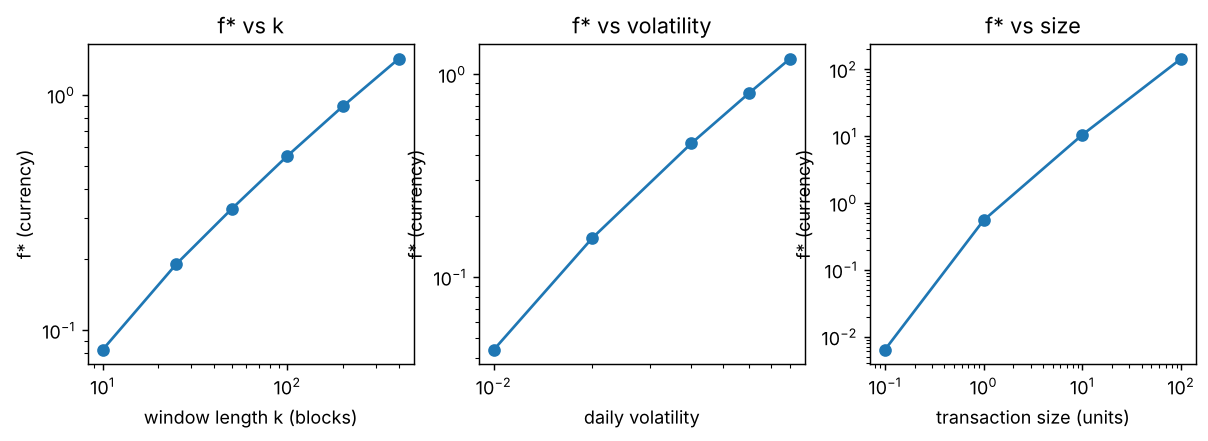
\includegraphics[width=0.92\linewidth]{assets/figs/course_fig_q1_sweeps}
\caption{$f^*$ in currency units against window, volatility and size.}\label{fig:q1}
\end{figure}

\begin{figure}[htbp]\centering
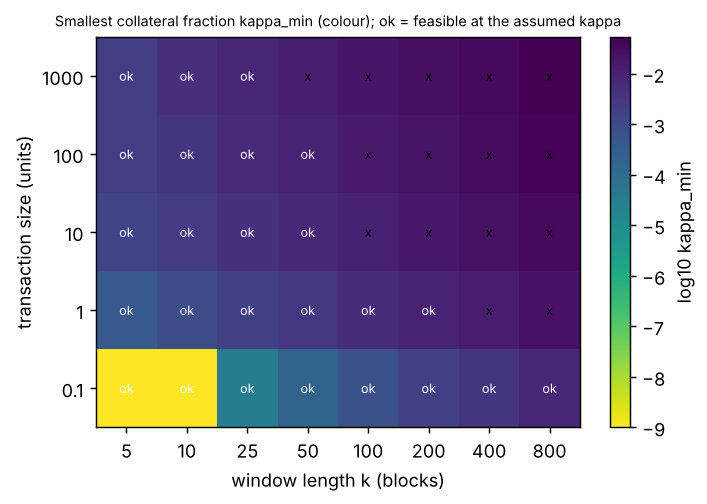
\includegraphics[width=0.55\linewidth]{assets/figs/course_fig_feasibility_map}
\caption{Smallest collateral fraction by window and size.}\label{fig:map}
\end{figure}

\begin{table}[htbp]\centering\footnotesize
\begin{tabularx}{\textwidth}{|>{\raggedright\arraybackslash}p{6.3cm}|Y|}
\hline
\rowcolor{gray!15}Check & Outcome \\
\hline
Hand-computed two-step game & $V_0=79/3$, and the solver gives \HandV \\
\hline
Separate game-tree solver, history-dependent strategies & agrees under every uniform tie-breaking rule, all three models \\
\hline
Exhaustive enumeration of pure strategies & agrees on small games, including the bonded contest \\
\hline
Centipede game & the unique subgame-perfect one of \CentNash\ Nash equilibria \\
\hline
Textbook binomial call pricing (Han et al.), no fee or forfeit & matches to within \HanMaxDiff \\
\hline
All-pay contest & indifference conditions and simulation confirm it \\
\hline
Automated test suite, with deliberately injected bugs & all \NTests\ tests pass, all \NMutants\ injected bugs caught \\
\hline
\end{tabularx}
\caption{Verification of the solver.}\label{tab:verify}
\end{table}

\begin{table}[htbp]\centering\footnotesize
\begin{tabular}{|l|r|r|c|}
\hline
\rowcolor{gray!15}Design & $f/f^*$ & speculator value (bp) & deterred? \\
\hline
plain commit-reveal (no forfeit) & 0.0 & 18.9 & No \\
\hline
forfeit only, small & 0.3 & 11.1 & No \\
\hline
forfeit only, large & 1.5 & $-3.3$ & Yes \\
\hline
fallback + burn & 0.3 & $-5.0$ & Yes \\
\hline
fallback + producer routing ($f>\mathrm{fee}-c$) & 0.3 & 11.1 & No \\
\hline
fallback + burn, signature $\Sigma$ optional & 0.3 & 11.1 & No \\
\hline
self routing & 1.5 & 18.9 & No \\
\hline
\end{tabular}

\caption{Speculator's value by design (bp).}\label{tab:q2}
\end{table}

\begin{table}[htbp]\centering\footnotesize
\begin{tabular}{|r|r|r|r|}
\hline
\rowcolor{gray!15}fee (bp) & fee at commitment (bp) & $f^*$ (lattice) & $f^*$ (closed form) \\
\hline
1 & 0 & 0.909\% & 0.917\% \\
\hline
2.5 & 0 & 0.711\% & 0.716\% \\
\hline
5 & 0 & 0.551\% & 0.554\% \\
\hline
10 & 0 & 0.387\% & 0.388\% \\
\hline
20 & 0 & 0.229\% & 0.229\% \\
\hline
5 & 2.5 & 0.429\% &  \\
\hline
5 & 5 & 0.337\% &  \\
\hline
5 & 10 & 0.193\% &  \\
\hline
\end{tabular}

\caption{Sensitivity of $f^*/N$ to the fee.}\label{tab:fee}
\end{table}

\begin{table}[htbp]\centering\footnotesize
\begin{tabular}{|l|r|r|r|}
\hline
\rowcolor{gray!15}Period & daily vol. & $f^*$ ($k{=}100$) & plain commit-reveal, speculator value (bp) \\
\hline
Pooled 2017--2026 & 4.57\% & 0.56\% & 18.9 \\
\hline
2018--2019 & 5.09\% & 0.65\% & 21.4 \\
\hline
2020--2021 & 5.61\% & 0.74\% & 23.8 \\
\hline
2022--2023 & 3.67\% & 0.41\% & 14.8 \\
\hline
2024--2026 & 3.53\% & 0.39\% & 14.1 \\
\hline
\end{tabular}

\caption{Volatility and $f^*$ by period.}\label{tab:periods}
\end{table}

\begin{table}[htbp]\centering\footnotesize
\begin{tabular}{|r|r|r|r|r|}
\hline
\rowcolor{gray!15}stake share $\alpha$ & $k=4$ & $k=8$ & $k=12$ & $k=20$ \\
\hline
0.1 & 1,000 & $>10^{6}$ & $>10^{6}$ & $>10^{6}$ \\
\hline
0.25 & 64.0 & 16,384 & $>10^{6}$ & $>10^{6}$ \\
\hline
0.5 & 8.0 & 128 & 2,048 & 524,288 \\
\hline
0.75 & 2.4 & 7.5 & 23.7 & 237 \\
\hline
0.9 & 1.4 & 2.1 & 3.2 & 7.4 \\
\hline
1 & 1.0 & 1.0 & 1.0 & 1.0 \\
\hline
\end{tabular}

\caption{Extortion threshold under rotating producers.}\label{tab:rot}
\end{table}

\begin{table}[htbp]\centering\footnotesize
\begin{tabular}{|l|r|r|r|r|r|}
\hline
\rowcolor{gray!15}routing & designs & P1 deters & P2 strict & P3 exact & all three \\
\hline
self & 300 & 300 & 300 & 0 & 0 \\
\hline
producer & 300 & 241 & 199 & 6 & 0 \\
\hline
mixed 50/50 & 300 & 238 & 211 & 9 & 0 \\
\hline
pool(4) & 300 & 244 & 215 & 15 & 0 \\
\hline
burn & 300 & 300 & 300 & 23 & 23 \\
\hline
\end{tabular}

\caption{Random search over designs.}\label{tab:imp}
\end{table}

\begin{table}[htbp]\centering\footnotesize
\begin{tabular}{|l|r|r|r|}
\hline
\rowcolor{gray!15}routing & threshold $\phi/\rho_P$ & first loss on grid at $f=$ & loss there \\
\hline
self & none & never & 0 \\
\hline
burn & none & never & 0 \\
\hline
pool(4) & 0.200\% & 0.257\% & 0.357\% \\
\hline
producer & 0.050\% & 0.064\% & 0.164\% \\
\hline
\end{tabular}

\caption{Extortion by a single strategic producer.}\label{tab:ext}
\end{table}

\begin{table}[htbp]\centering\footnotesize
\resizebox{\linewidth}{!}{\begin{tabular}{|r|r|r|r|r|r|r|}
\hline
\rowcolor{gray!15}$q$ & 99\% rule$/f^*$ & 95\% rule$/f^*$ & exact minimiser$/f^*$ & participation (99\% rule) & loss at $f{=}0$ (bp) & loss at 99\% rule (bp) \\
\hline
0.05 & 2.14 & 1.32 & 6.75 & 0.45 & 12.80 & 0.13 \\
\hline
0.3 & 2.12 & 1.30 & 7.00 & 0.45 & 12.66 & 0.13 \\
\hline
0.6 & 2.03 & 1.25 & 5.50 & 0.45 & 12.36 & 0.12 \\
\hline
\end{tabular}
}
\caption{Designer's forfeit with a private user type.}\label{tab:bp}
\end{table}

\begin{table}[htbp]\centering\footnotesize
\resizebox{\linewidth}{!}{\begin{tabular}{|r|r|r|r|r|}
\hline
\rowcolor{gray!15}size & $f^*/N$, flat fee & $f^*/N$, fee $\propto$ size & speculator value, rule calibrated at size 1 (bp) & speculator value, line through the sizes (bp) \\
\hline
0.1 & 0.064\% & 0.551\% & $-31.1$ & $-49.2$ \\
\hline
1 & 0.551\% & 0.551\% & 0.0 & $-4.9$ \\
\hline
10 & 1.048\% & 0.551\% & 3.8 & $-0.5$ \\
\hline
100 & 1.443\% & 0.551\% & 4.2 & 0.0 \\
\hline
\end{tabular}
}
\caption{Forfeits that grow with transaction size.}\label{tab:size}
\end{table}
\begin{table}[htbp]\centering\footnotesize
\begin{tabular}{|r|r|c|c|r|c|}
\hline
\rowcolor{gray!15}$a$ & $V_a/V_o$ & race deters? & attack cost to deter race & smallest bond & bond deters? \\
\hline
0.5 & 0.5 & No & 0.250 & 0.480 & Yes \\
\hline
0.5 & 1 & No & 0.500 & 0.980 & Yes \\
\hline
0.5 & 2 & No & 1.500 & n/a & no (bond $>K$) \\
\hline
0.8 & 0.5 & No & 0.100 & 0.113 & Yes \\
\hline
0.8 & 1 & No & 0.200 & 0.238 & Yes \\
\hline
0.8 & 2 & No & 1.200 & 0.488 & Yes \\
\hline
0.9 & 0.5 & No & 0.050 & 0.045 & Yes \\
\hline
0.9 & 1 & No & 0.100 & 0.100 & Yes \\
\hline
0.9 & 2 & No & 1.100 & 0.212 & Yes \\
\hline
0.99 & 0.5 & Yes & 0.005 & 0.000 & Yes \\
\hline
0.99 & 1 & Yes (tie) & 0.010 & 0.000 & Yes \\
\hline
0.99 & 2 & No & 1.010 & 0.011 & Yes \\
\hline
\end{tabular}

\caption{Race against bond ($V_o=\ContestVo$, $\kappa=\ContestKappa$, $c_r=\ContestCr$, $K=\ContestCap$).}\label{tab:contest}
\end{table}

\begin{table}[htbp]\centering\footnotesize
\begin{tabular}{|r|c|c|c|}
\hline
\rowcolor{gray!15}$k$ & daily vol.\ 2.00\% & daily vol.\ 4.57\% & daily vol.\ 8.00\% \\
\hline
10 & 0.02 / 0.13 & 0.09 / 0.34 & 0.22 / 0.67 \\
\hline
25 & 0.05 / 0.23 & 0.20 / 0.60 & 0.45 / 1.15$^{\ast}$ \\
\hline
50 & 0.09 / 0.35 & 0.33 / 0.91 & 0.74 / 1.69$^{\ast}$ \\
\hline
100 & 0.16 / 0.53 & 0.56 / 1.35$^{\ast}$ & 1.20 / 2.50$^{\ast}$ \\
\hline
200 & 0.28 / 0.79 & 0.90 / 1.98$^{\ast}$ & 1.88 / 3.66$^{\ast}$ \\
\hline
\end{tabular}

\caption{$f^*$ and $f_{\mathrm{cp}}$ by window and volatility.}\label{tab:burnrange}
\end{table}

\begin{table}[htbp]\centering\footnotesize
\begin{tabular}{|r|r|r|r|}
\hline
\rowcolor{gray!15}tolerance (bp) & $f_{\mathrm{cp}}$ at $k{=}100$ & largest $k$ within 1\% & minutes \\
\hline
1 & 0.91\% & 117 & 23.4 \\
\hline
0.1 & 1.35\% & 59 & 11.8 \\
\hline
0.01 & 1.69\% & 39 & 7.8 \\
\hline
0.001 & 1.99\% & 29 & 5.8 \\
\hline
\end{tabular}

\caption{Sensitivity to the coalition-gain tolerance.}\label{tab:tol}
\end{table}

\begin{table}[htbp]\centering\footnotesize
\begin{tabular}{|l|c|r|r|r|}
\hline
\rowcolor{gray!15}routing & producer publishes? & gain at 0.5$f^*$ (bp) & gain at 1$f^*$ (bp) & gain at 3$f^*$ (bp) \\
\hline
burn & Yes & 10.44 & 4.22 & 0.01 \\
\hline
self & Yes & 21.43 & 21.43 & 21.43 \\
\hline
pool(4) & No & 0.00 & 0.40 & 0.12 \\
\hline
producer & No & 1.66 & 8.51 & 21.22 \\
\hline
\end{tabular}

\caption{Coalition gain by routing (bp).}\label{tab:coal}
\end{table}

\begin{table}[htbp]\centering\footnotesize
\begin{tabular}{|r|r|r|}
\hline
\rowcolor{gray!15}$q$ & $f^*/N$ & speculator value without a forfeit (bp) \\
\hline
0 & 0.551\% & 18.9 \\
\hline
0.1 & 0.551\% & 18.9 \\
\hline
0.3 & 0.549\% & 18.9 \\
\hline
0.6 & 0.540\% & 18.7 \\
\hline
0.9 & 0.475\% & 17.3 \\
\hline
\end{tabular}

\caption{$f^*$ against the censoring probability.}\label{tab:qsweep}
\end{table}
\begin{table}[htbp]\centering\footnotesize
\begin{tabular}{|r|r|r|r|}
\hline
\rowcolor{gray!15}daily vol. & Han method (\%) & game solver (\%) & $|$diff$|$ \\
\hline
0.75\% & 0.2971 & 0.2971 & 8.1e-14 \\
\hline
2.00\% & 0.7924 & 0.7924 & 1.1e-13 \\
\hline
3.00\% & 1.1885 & 1.1885 & 9.0e-14 \\
\hline
4.00\% & 1.5846 & 1.5846 & 8.3e-14 \\
\hline
5.00\% & 1.9807 & 1.9807 & 2.8e-14 \\
\hline
5.80\% & 2.2975 & 2.2975 & 1.2e-14 \\
\hline
\end{tabular}

\caption{Binomial premium against the game solver.}\label{tab:han}
\end{table}
\begin{table}[htbp]\centering\footnotesize
\begin{tabular}{|r|r|r|r|r|}
\hline
\rowcolor{gray!15}multiple $m$ (12 s) & VR($m$) & $z$ & robust $z$ & implied exponent \\
\hline
2 & 1.049 & 15.5 & 4.8 & 0.534 \\
\hline
5 & 1.093 & 13.4 & 4.7 & 0.528 \\
\hline
10 & 1.108 & 10.1 & 3.9 & 0.522 \\
\hline
25 & 1.093 & 5.3 & 2.3 & 0.514 \\
\hline
50 & 1.091 & 3.6 & 1.7 & 0.511 \\
\hline
100 & 1.084 & 2.3 & 1.2 & 0.509 \\
\hline
300 & 1.083 & 1.3 & 0.8 & 0.507 \\
\hline
\end{tabular}

\caption{Variance ratios of 12-second returns.}\label{tab:vr12}
\end{table}
\begin{table}[htbp]\centering\footnotesize
\begin{tabular}{|r|r|r|r|r|}
\hline
\rowcolor{gray!15}multiple $m$ & VR($m$) & $z$ & robust $z$ & implied exponent \\
\hline
2 & 1.006 & 1.8 & 0.3 & 0.504 \\
\hline
5 & 1.001 & 0.1 & 0.0 & 0.500 \\
\hline
10 & 0.978 & -1.9 & -0.4 & 0.495 \\
\hline
30 & 1.000 & 0.0 & 0.0 & 0.500 \\
\hline
60 & 1.005 & 0.2 & 0.1 & 0.501 \\
\hline
\end{tabular}

\caption{Variance ratios of one-minute returns.}\label{tab:vr}
\end{table}
\begin{table}[htbp]\centering\footnotesize
\begin{tabular}{|l|r|r|r|}
\hline
\rowcolor{gray!15}asset & daily vol. & 95\% interval & $f^*$ ($k{=}100$) \\
\hline
ETHUSDT & 4.57\% & 4.23\%--4.98\% & 0.56\% \\
\hline
BTCUSDT & 3.53\% & 3.25\%--3.89\% & 0.39\% \\
\hline
SOLUSDT & 5.95\% & 5.38\%--6.63\% & 0.80\% \\
\hline
BNBUSDT & 4.90\% & 4.28\%--5.56\% & 0.61\% \\
\hline
\end{tabular}

\caption{Calibration and $f^*$ by asset.}\label{tab:assets}
\end{table}


\clearpage
\section{Additional Results}\label{app:extra}
\textbf{Unknown user types.} When a share $\pi$ of users are speculators ($k=\DesignerK$, $f^*=\DesFstarBp$ bp), full deterrence is optimal in \DesFull\ of the 36 combinations of $(q,\pi)$ tested, since an honest user is dropped with probability $q^{k-1}<10^{-6}$ even at $q=0.7$.

\textbf{Private user types.} In the private-type model of Section~\ref{sec:model}, moderately exposed users also exploit the delay. The designer's forfeit under the 99\% loss-reduction rule is \BPLow\ to \BPHigh\ times $f^*$ across the $q$ tested, and \BPSensLo\ to \BPSensHi\ when the prior is varied (Table~\ref{tab:bp}). These factors depend on the illustrative prior and objective.

\textbf{Nash equilibria and subgame perfection.} The verification tools also show why the solution concept of Section~\ref{sec:model} matters. With a burned forfeit of $50$ in illustrative units and a fallback, only \BurnSPNE\ of \BurnNash\ pure Nash equilibria are subgame perfect, and the other \BurnNonCred\ rest on a producer threat to withhold that it would never carry out.

\textbf{Gaussian approximation.} If $g_{k-1}$ is roughly normal with standard deviation $s$, the put in Proposition~\ref{prop:value} costs $a\Phi(a/s)+s\,n(a/s)$ with $a=\phi-f$, where $\Phi$ and $n$ are the standard normal distribution function and density. This is a closed-form expression for the put, not for $f^*$, and solving it equal to $\phi$ numerically gives an approximation to $f^*$, compared with the lattice in Table~\ref{tab:fee}.

\textbf{Fee paid at commitment.} A fee paid at commitment lowers the speculator's value by a constant, and one of $5$ bp lowers $f^*$ from \FstarKHundred\ to \CommitFeeFive\ (Table~\ref{tab:fee}).

\textbf{Forfeits that grow with size.} Under the flat fee, a forfeit proportional to size and calibrated at size one leaves a speculator \SizePropMaxResidual\ bp at size $100$. A forfeit fitted as a line across sizes over-penalizes the smallest trades \SizeLineOverSmall\ times (Table~\ref{tab:size}).

\textbf{Loss function of the private-type model.} Here all money is divided by $N$, which is the same as setting $N=1$, so a type's extra value from execution is $\theta$. A type commits if its best-response value $V_{\mathrm{br}}$ is at least zero, and $V_{\mathrm{hon}}$ is its value of authorizing at once. Its \emph{option-exploitation benefit} is $X=V_{\mathrm{br}}-V_{\mathrm{hon}}$, the gain from timing its authorization instead of authorizing at once, and it bears a friction $F=(\theta-\phi)-V_{\mathrm{hon}}$, while a deterred type loses its surplus $s(\theta)=\max(\theta-\phi,0)$. The designer minimizes $L(f)=\E_\theta[\mathbf 1_{\text{commit}}(\lambda X+\nu F)+\mathbf 1_{\text{deterred}}\,s(\theta)]$, where $\E_\theta$ averages over the type distribution and $\lambda$ and $\nu$ weight exploitation and friction. $X$ is a chosen proxy for harm to counterparties, not a measured loss. With $q=0$, for example, $X=\E[g_\tau\mathbf 1_{\text{exec}}]-(\theta-\phi+f)\Pr(\text{drop})$, where the first term is the counterparty's trading loss and the second is the user's own change in fees, forfeits and execution, so $X$ equals neither the counterparty's loss nor a welfare loss in general. The near-flatness of $L$ once exploitation vanishes motivates the loss-reduction rules defined before Table~\ref{tab:bp}.

\textbf{Prior of the private-type model.} The prior puts weights $0.35$, $0.20$, $0.15$, $0.12$, $0.08$, $0.06$ and $0.04$ on exposures of $0$, $2$, $5$, $10$, $20$, $50$ and $100$ bp, and the loss weights are $\lambda=\nu=1$.

\textbf{Exact minimiser of the private-type loss.} The exact minimiser rises from \BPExactCoarse\ to \BPExactFine\ times $f^*$ as the number of steps in the window rises from \BPStepsLow\ to \BPStepsHigh\ with the window's volatility held fixed. This is a joint sensitivity and not a pure refinement, because each extra step is also an extra authorization attempt with the same censoring probability $q$, so at $q=0.6$ the chance that every attempt fails falls from $0.6^{5}\approx0.078$ to $0.6^{80}\approx2\times10^{-18}$. A pure refinement would subdivide the price steps while keeping the authorization schedule, which is left for future work. The baseline at $k=\DesignerK$ is unaffected. The 99\% rule is steadier. It is refined between coarse grid points, with the target taken from the coarse-grid minimum, and it gives \BPEpsFineLow\ to \BPEpsFine\ times $f^*$ on the finest lattice. A forfeit grid with spacing $0.25f^*$ gives \BPGridCoarse\ and one with spacing $0.025f^*$ gives \BPGridFine.

\textbf{Intraday checks of the price model.} The 12-second data are 14 days of one-second ETH closes, \TwFrom\ to \TwTo, resampled to 12-second blocks, which gives \TwN\ overlapping \EmpWindow-minute windows. The realized volatility per block is \TwSigmaStep\ against \TwImpliedStep\ implied by the full-history calibration, a daily equivalent of \TwDailyEq, so the forfeits in the main text belong to a more volatile regime. The variance ratio is \TwVRTwo\ at 24 seconds and between \TwVRLow\ and \TwVRHigh\ at longer horizons (Table~\ref{tab:vr12}). A test that is robust to changing volatility finds it above one at the pointwise 5\% level only up to about \TwSigMinutes\ minutes ($z=\TwZRobShort$ at 24 seconds and \TwZRobSig\ at \TwSigMinutes\ minutes) and not at 20 minutes ($z=\TwZRobWindow$), with no correction for the number of horizons. The point estimate is that square-root-of-time scaling understates the window's standard deviation by about \TwUnderstate, which this sample cannot tell apart from zero. The empirical forfeit and $95\%$ interval reported in Section~\ref{sec:discussion} use \TwNBoot\ block-bootstrap resamples (seed \TwSeed, blocks twelve windows long). The one-minute data run from \EmpFrom\ to \EmpTo. There the interval \EmpCI\ excludes the lognormal value of \EmpLognormal\ (ratio \EmpRatio).

\section{Reproducing the Results}
The repository \repo\ contains the code, the price data and every result file. After installing the packages in \verb|requirements.txt|, the single command \verb|./run_all.sh| runs the tests, regenerates every result and rebuilds this report from the data in the repository (about 25 minutes). It uses only the frozen price data committed in \verb|data/| and stops at the first failing step. The command \verb|python scripts/compare_results.py| then checks every regenerated CSV file, staged or not, against the committed one, treating a changed NaN or a sign change of an infinity as a real difference. The pipeline was tested with Python 3.12 and TeX Live 2023, and \verb|docs/REPRODUCING.md| lists the LaTeX packages needed. Setting \verb|REFRESH_DATA=1| when running \verb|scripts/run_assets.sh| downloads newer prices for the asset comparison and therefore changes those results. Results are written to \verb|results/|, with the main calibration in \verb|results/main/|. The individual steps are as follows.
\begin{itemize}\small
\item \verb|python -m pytest| runs the automated tests.
\item \verb|python scripts/run_project.py| produces every table and figure for the main calibration.
\item \verb|python scripts/run_extras.py| produces the sensitivity and range analyses.
\item \verb|python scripts/run_course_core.py| produces the verification facts.
\item \verb|./scripts/run_periods.sh| and \verb|./scripts/run_assets.sh| produce the period and asset comparisons.
\item The one-minute checks and the 12-second checks come from the two commands below.
\begin{verbatim}
python scripts/run_empirical.py --data data/ETHUSDT_1m.csv
python scripts/run_empirical.py --data data/ETHUSDT_12s.csv \
  --window-minutes 20 --vr-multiples 2 5 10 25 50 100 300 \
  --n-boot 1000 --block-windows 12 --seed 0 --out results/intraday_12s
\end{verbatim}
\item \verb|python scripts/make_report_assets.py| writes the tables and numbers used by this report.
\end{itemize}
\end{document}
